% This is a thesis template that attempts to conform to the guidelines
% published by UTRGV's Graduate School office.

% Please report any issues to
% https://github.com/UTRGV-SMSS/Thesis-Template/issues

% The author of this template is Guillermo Garza.


% Switch this line to the final option when submitting your thesis.
% This will correct counts and remove labels that are shown during draft mode

\documentclass[12pt,masters,final]{UTRGVthesis}

%\documentclass[masters,final]{UTRGVthesis}
%\documentclass[masters,final, nodedication, noacknowledgments]{UTRGVthesis}


% Load your packages below.
% Make hyperref and showkeys come at the end of your loaded packages
% to make sure they are not over-written.  They redefine many
% standard LaTeX commands

\usepackage{docmute} % for inputting complete documents. Useful for LyX users
\usepackage{booktabs} % for better tables
\usepackage{microtype} % for better typography
\usepackage[colorlinks=false]{hyperref}  % for urls

%\usepackage{showkeys} % shows labels during draft mode
\usepackage[document]{ragged2e} % uncomment for non-justified text

\usepackage{mwe}
\usepackage{graphicx}
\usepackage{floatrow}
\usepackage{flexisym}
\usepackage{tikz}
\usepackage{amsmath}
\usepackage{subcaption}
\usepackage{makecell}

%\usepackage{Times}
%\usepackage{mathptmx}
\usepackage{fontspec}
\setmainfont{Times New Roman}
%\setmainfont[Mapping=tex-text]{Times New Roman}
%\usepackage[T1]{fontenc}
%\usepackage[utf8]{inputenc}
% For indentation after one line in Bibliography
\usepackage[sort&compress]{natbib}      % for bibliography

\setlength\bibindent{2em}

\makeatletter
\renewcommand\NAT@bibsetnum[1]{\settowidth\labelwidth{\@biblabel{#1}}%
   \setlength{\leftmargin}{\bibindent}\addtolength{\leftmargin}{\dimexpr\labelwidth+\labelsep\relax}%
   \setlength{\itemindent}{-\bibindent}%
   \setlength{\listparindent}{\itemindent}
\setlength{\itemsep}{\bibsep}\setlength{\parsep}{\z@}%
   \ifNAT@openbib
     \addtolength{\leftmargin}{\bibindent}%
     \setlength{\itemindent}{-\bibindent}%
     \setlength{\listparindent}{\itemindent}%
     \setlength{\parsep}{0pt}%
   \fi
}
\makeatother
% Uncomment the line below to check if text is aligned to margins
%\margins
% this sets the name of the bibliography
% add \vspace{1cm} here to adjust vertical spacing after bibliography title
\renewcommand{\bibname}{REFERENCES}


% Insert your name and major here in the format shown
\Author{Pawan Kumar Thapaliya }
\AuthorLastFirst{Thapaliya, Pawan}
\Major{Physics}


% Insert your graduation date here
\Month{July}
\Year{2019}


% Insert the title of your thesis here.
% If you have a long title, split it between multiple lines using the \\ command
% Also, use comment characters to avoid unwanted spaces in the Abstract page
\Title{Bubble Nucleation And Cooperativity in Duplex Stretching of a Helicoidal DNA Model}


% Insert your research advisor and his title here
\Advisor{Dr. Andreas Hanke}
\AdvisorTitle{Chair of Committee}


% Insert the members of your committee here
% You can also give MemberA a special title
\MemberA{Dr. Ahmed Touhami}  %\MemberATitle{Co-Chair of Committee}
\MemberB{Dr. Hyeongjun Kim}
\MemberC{}
\MemberD{}
\MemberE{}


% Insert the text of your abstract below.
% The bibliography style "citation" required by the manual is automatically
% generated.  Specify the "final" option in the \documentclass to update the
% counts to the correct values.
%\vspace{1cm}
\Abstract{Denaturation of DNA means separation of dsDNA into ssDNA due to the breaking of hydrogen bond by the application of heat or another mechanical method to carry out the processes like translation,transcription, and replication. Single-molecule DNA stretching experiments displayed a force-induced transition at a force of 65pN for long dsDNA molecules. In these experiments, double-stranded DNA molecules are stretched by a force applied to opposite ends of the DNA, e.g., in anatomic force microscope or an optical tweezers instrument. Here we study the thermal and force-induced denaturations of the helicoidal DNA bubble-in-the-middle sequence by Monte-Carlo simulations technique. We applied periodic boundary conditions to avoid a large number of opening at the ends of the DNA molecules. Our goal is to quantitatively predict DNA melting curves for short DNA (10-100  sequence of base pairs) and to show that statistical physics can be used to understand the stretching behavior of short DNA oligomer. We compare the results of our simulations with the previously published experimental result for both thermal and mechanical DNA stretching.}


% You can dedicate your paper here.  This is optional.
\Dedication{I wish to dedicate this work to my late father Madhu Sudan Thapaliya and my mother Om Kumari Thapaliya. They inspired me to be an educated person.}


% Acknowledge those who helped and supported you here. This is optional.

\Acknowledgments{I would like to express my sincere gratitude to my supervisor Andreas Hanke, who groomed me from the very beginning of the project. Without his help, I could not have reached this stage. Under his supervision, I got opportunities to improve myself and removed my weakness. I am also thankful to my wife Ranjana Pokharel and son Rawan Kumar Thapaliya whose presence around me always motivated me to put hard effort. At last, I am also overwhelmed by the constant encouragement from relatives and friends whose valuable word always boosted me to stay in front of the computer all day.}


% Insert your biographical sketch here.

\BiographicalSketch{Pawan Kumar Thapalia was born in 11/30/1985 at Nuwakot,Nepal. He was one of the bright student since his high school. He finished his Undergradaute and Gradaute degree from Tribhuvan University Nepal on 2009 and 2011. \\
From Fall 2016-Summer 2019 he had worked as a Research and Teaching assistant at Department of Physics University of Texas Rio Grande Valley . He received his Master in Science degree in  July 2019. He is available in the following addresses:\\
Email: pawanthapaliya09@gmail.com\\
Phone:4695315525 }


\begin{document}

% This starts page counting in Roman numerals
\frontmatter


% This command makes the formal preliminary pages.
% You can comment it out during the drafting process if you want to save paper.
\makepreliminarypages


% These insert a table of contents, list of tables, and list of figures
\tableofcontents

\listoftables      
\listoffigures      %List of figures displays scambled figure captions

% This starts regular page counting in Arabic numerals
\mainmatter

% This starts double-spaced text.  Opposite command is \singlespacing
\doublespacing

% define \angstrom in math mode
\newcommand{\angstrom}{\text{\normalfont\AA}}

% OK. Everything is set up. Insert your thesis below.
% It's a good idea to split your thesis up into different files and use
% the \input command
\chapter{Introduction}
\section{DNA}
Deoxyribonucleic acid, in short, is the double-stranded helical molecule which is considered as the carrier of genetic information. Structurally DNA is made up of sugar, phosphate and Nitrogen Bases. According to the Watson Crick model~\cite{watson1953structure} Sugar and Phosphate made outer backbone length whereas bases are locked inside by hydrogen bond. Bases are classified as Purine( Adenine and Guanine) and Pyrimidine( Thyamine and Cytosine). Fig.~\ref{fig:DNA structure} shows that the two strands of DNA are complementary to each other start from 5' to 3' end. The bases are paired as AT and GC. The bond structure of AT is little flexible due to stacking interaction and two hydrogen bonds present between them than that of the GC which is stronger due to three hydrogen bonds present between its bases and the strong interaction along with the bases of the same strand.The pieces of information are stored in the sequence of base pairs at the two strands of DNA ~\cite{Calladine:2004, hanke2013denaturation}. These pieces of information are transformed during replication, transcription, and translation.\\
%
\indent
The covalent bond (strength about $100 kcal/mole$) along the sugar-phosphate backbone, the hydrogen bond (strength about $5 kcal/mole$) present between the nitrogen bases of a complementary strand in large number is responsible for stabilizing the DNA helix. Other forces responsible for DNA stability are the stacking interaction which is accounted by Hydrophobic effects of bases in water solution, London dispersion forces, Van der Waals interaction (about $0.5 kcal/mole$) and dipole-dipole interaction. These forces result in a complex interaction pattern between overlapping base pairs, with minimum energy distance close to 3.4 Å in the normal DNA double helix. The bases are hydrophobic in nature whereas sugar and phosphate are hydrophilic
in nature. So to avoid contact with water, bases are locked inside by sugar and Phosphate groups giving a more stable double helix structure. The stacked bases attracted each other through Van der Waals force of attraction. These attractions are between the $\pi$ electron cloud of the bases of the same strand. Charge-Charge Interactions is responsible for  the electrostatic (ion-ion) repulsion of the negatively charged phosphate which makes the DNA helix potentially unstable, but the presence of $Mg_{2}^{+}$ and cationic proteins with abundant  Arginine and Lysine residues reduce
the repulsive effects and stabilize the molecules~\cite{sugimoto1996improved,ivanov2004statistical}.
%
\newpage
%
\begin{figure}[!h]
  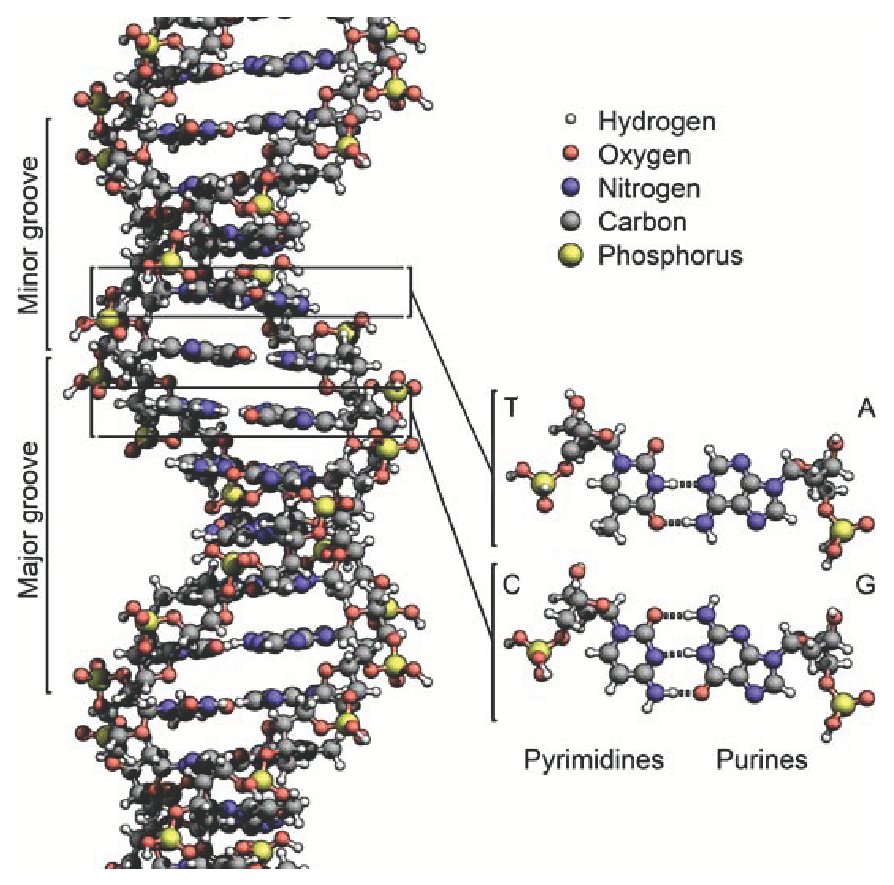
\includegraphics[height=6in,width=1 \textwidth]{dna_structure.eps}
  \floatsetup[figure]{font=1}
  \caption{\small The Watson-Crick DNA~\protect\cite{watson1953structure}: structure: The figure represents the sugar-phosphate backbone length along the strand and pairing of complimentary Purines and Pirimidines bases. The image was designed by Zephyris taken from Wikimedia Commons\,. }
  \label{fig:DNA structure}
\end{figure}
%
\newpage
\section{DNA denaturation by heating and stretching}
\subsection{DNA denaturations by heating}
Under physiological conditions, the B-form double helix is considered as the most thermodynamically stable configuration of DNA. However, the local opening of DNA duplex is required to accomplish the phenomenon like replication, transcription, and translation~\cite{Alberts:2015}. Thermal denaturation also called melting is one of the experimental methods to separate the double-stranded DNA to single-stranded  DNA by heating. During this experiment, dsDNA is kept at UV light at 260 nm. The increase in absorbance of UV light indicates that ds DNA denatures to ssDNA~\cite{peyrard2004nonlinear,dauxois1995entropy}. Fig.\ref{fig:DNA thermal melting} reflects that upon heating double-stranded DNA, regions of unbound base pairs proliferate along the molecule due to thermal fluctuations at the thermal melting temperature, $ i.e.$ temperature at which half of the DNA is believed to be denatured. For the heteropolymer, the denaturations depend on the concentration of AT and GC. The rate of melting is inversely proportional to the GC concentration. Depending of GC concentration $T_m \sim 60^{\circ} - 90$\,$^{\circ}$ Celsius~\cite{DB:1991}. Over a narrow range of temperatures near $T_m$ the fraction of bound base pairs decreases from one to zero as the two strands separate
in a process called DNA denaturation or melting~\cite{Wartell:1985}.
\begin{figure}[!h]
  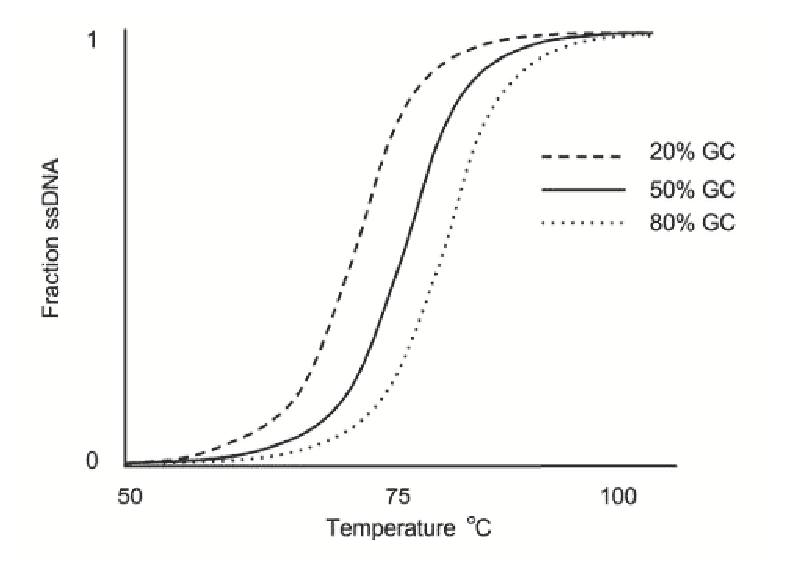
\includegraphics[width=0.65 \textwidth]{dna_thermal_melting.eps}
  \floatsetup[figure]{font=1}
  \caption{\small Experimental DNA melting curves for long DNA molecules with different levels of GC content.The y-axis indicates the fraction of DNA molecules that are single-stranded.This curve is taken from online source of Khan Academy \,. }
  \label{fig:DNA thermal melting}
\end{figure}
%
\newpage
\subsection{DNA denaturations by stretching}
Apart from heating, DNA denaturation can be observed through the application of mechanical stress to the DNA molecules. The development of optical tweezers, magnetic tweezers, and atomic force microscopes enabled the stretching and twisting activities on DNA molecules  in the Biophysics experiment~\cite{Strick:2003}. In these experiments, the tip of one end of the DNA is chemically anchored to a surface and the sensor attached to the other end measures the applied force. In optical or magnetic tweezer instruments the sensor is a microbead whereas in an atomic force microscope (AFM) the sensor is a microscopic cantilever, as shown in Fig.\ref{fig:DNA stretching}. The force versus extension curve obtained from the measurement helps to understand the mechanical properties of DNA.\\ 

\indent
DNA stretching experiments are applicable to study long DNA molecules, such as phage-$\lambda$ DNA ($\sim 50,000$ bp). In this experiment the DNA is coupled between two polystyrene beads and the force $F$ on the DNA is calculated as a function of the DNA extension~\cite{Smith:1996, CS:2000, Strick:2003, C:2010}. When long DNA molecules are extended beyond their B-form contour length a structural transition occurs during which the extension $L$ of the DNA increases to almost twice its B-form contour length over a very small force range. The transition is called B-S transition because in this range the bound DNA is converted to stretched DNA.The observed force-extension relations $F(L)$ demonstrates the plateau at forces of $F_m \sim 65$\,pN where the DNA extension per base pair increases from 0.34 to about 0.55 $nm$ (Fig.\ref{fig:DNA overstretching})~\cite{Smith:1996, CS:2000, Strick:2003, C:2010}. The length of the plateau determines the cooperativity of the DNA. DNA molecules having large plateau length are considered more cooperative than the one having short plateau length. It was indicated that at $F_m$ the DNA undergoes a force-induced melting transition where double-stranded DNA is progressively converted to single-stranded DNA, in close analogy to thermal melting of free DNA at the thermal melting temperature~\cite{C:2010}. This model can be used to quantitatively explain the thermodynamics of DNA overstretching as a function of solution conditions and in the presence of DNA binding ligands, and is supported by a 
large number of experimental observations~\cite{C:2010}. 
%
\begin{figure}[!h]
  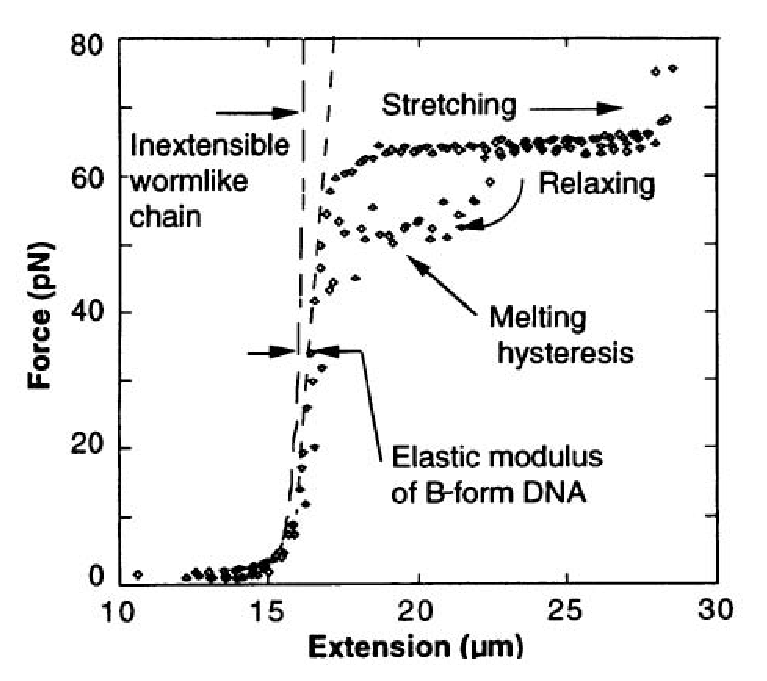
\includegraphics[width=0.5 \textwidth]{dna_overstretching.eps}
  \floatsetup[figure]{font=1}
  \caption{\small Experimental force-extension relation for phage-$\lambda$ DNA. When the molecule is stretched beyond its B-form contour length it shows a highly cooperative overstertching transition at 65 pN where the DNA extension increases by a factor of 1.7 with very little force increase. The transition is interpreted as force-induced melting where double-stranded DNA is gradually converted to single-stranded DNA as the DNA extension is increased~\protect\cite{Smith:1996}.}
  \label{fig:DNA overstretching}
\end{figure}
%
\newpage

A large variety of stretching experiments have also been done on short DNA oligomers a few tensof base pairs in length; see, e.g.,~\cite{Strunz:1999, Pope:2001, Morfill:2007}. In these experiments, the two strands of the duplex dissociate at considerably lower forces of about 30 pN than the force $\sim 65$\,pN at the overstretching plateau observed for long DNA. Moreover, the observed rupture forces depend on the pulling rate, i.e., the speed with which the DNA is stretched. We apply the Monte Carlo simulation technique to understand the stretching behavior of the short DNA oligomer.
%
\newpage
\chapter{Method}
%
\section{Peyrard-Bishop model for helicoidal DNA}
At large scale, theoretical model-that uses self-avoiding walks to understand two strands of DNA helicoid, are successful to explore the properties of the melting transition~\cite{martin2000localization,kafri2000dna,carlon2002roles}. However, they cannot be convincing method to investigate sequence or probe dependent properties of DNA at microscopic scale like some recent single-molecule experiment because they ignore the DNA at base pairs level. In such situations model like Peyrard-Bishop(PB) model~\cite{peyrard1989statistical} which cover the scale of the base pair is useful. The reasonable explanation of hydrogen bond interaction between the complementary strand and the staking interaction within the strand makes the model handy tools for understanding the complex DNA strand. In this model, bases in the opposite strand are constrained to move only in the direction of hydrogen bond connected by Morse potential representing hydrogen bonds, on the other hand, bases in the same strand are coupled harmonically. Local melting of the hydrogen bond and formation of denaturations bubbles are the special features of this model\\
\indent
As PB model discuss one dimensional DNA and missed the helicoidal structure of it. There require an extended PB model that considers the helical structure of DNA. This weakness is removed in the helicoidal model of DNA. So far there has been proposed two kinds of helicoidal model. The first one~\cite{barbi2003thermal} considers the fixed base planes and elastic backbones whereas the second~\cite{cocco1999statistical} one considers the varying base planes and fixed backbones. Both models agree to give similar result because they both address the coupling between opening and twist that results from the helicoidal geometry.\\
\indent
\begin{figure}[!h]
  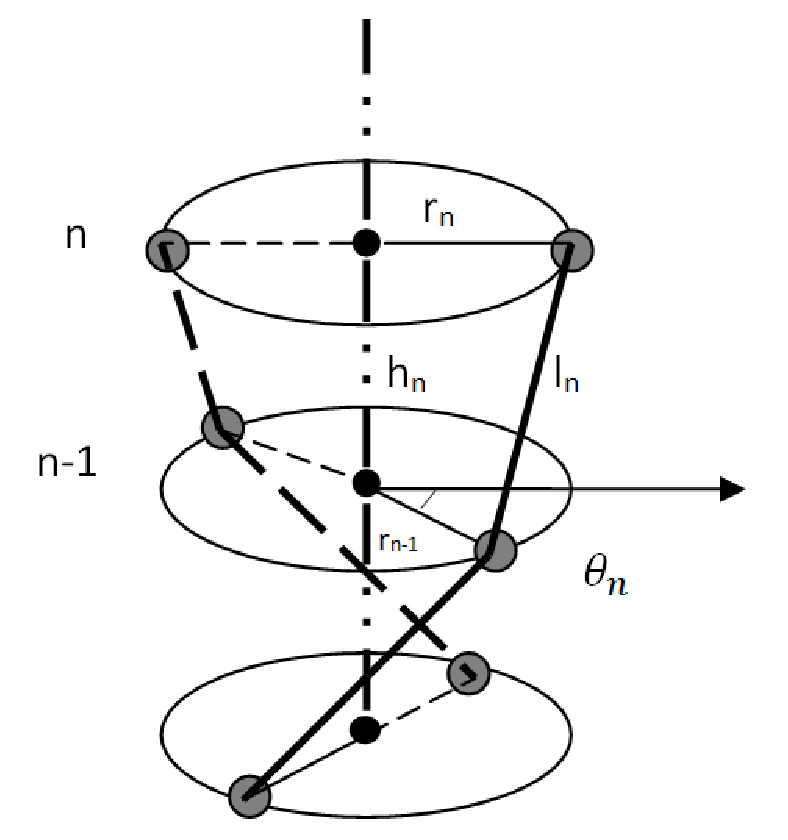
\includegraphics[width=0.5 \textwidth]{DNA_helicoid.eps}
  \floatsetup[figure]{font=1}
  \caption{\small Helicoidal Model~\protect\cite{peyrard2004nonlinear} $r_{n}$ and $\phi_{n}$ determines the base pair positions in the plane. Axial distance $h_{n}$ varies as a function of $r_{n},\theta_{n}$, and $l_{n}$. We  reproduce the figure of~\protect\cite{cocco1999statistical} with necessary updates to fit our model\,. }
  \label{fig:Helical Structure}
\end{figure}

At ambient  temperature $T = 300^\circ$K and without stretching force $f$, our model reproduces the Watson-Crick double helix of B-form DNA as shown in Fig.~\ref{fig:Helical Structure}. We consider a chain of $N$ base pairs numbered by $n = 1,\ldots,N$.
Each base pair is constrained to move in a plane perpendicular to the helical axis. We assume that the two bases in each base pair $n$ move about the helical axis symmetrically, i.e., they have the same radial distance $r_n$ from the helical axis (and thus distance $2 r_n$ from each other).
The position of base pair $n$ in base pair plane $n$ is described by the radial and angular position $r_n$ and $\phi_n$ in the plane.
The local twist angle of base pair $n$ relative to base pair $n-1$ is given by
$\theta_n = \phi_n - \phi_{n-1}$. Subsequent base pair planes $n-1$ and $n$ have a variable rise $h_n$ along the helical axis. To impose the helical structure of B-form DNA, we assume that bases $n-1$ and $n$ are connected by a flexible sugar phosphate backbone segment of length $l_n > h_n$ along each strand, so that the ratio $l_n / h_n > 1$ gives the helicity at base pair $n$ (Fig.~\ref{fig:Helical Structure}).
A particular conformation of the DNA molecule is thus completely specified (up to a rigid rotation of the whole molecule about the helical axis) by the set of variables
%
\begin{equation} \label{variables}
  \{r_n, \theta_n, l_n\} := \{(r_n, \theta_n, l_n), \, \, n = 1,\ldots,N\} \, \, .
\end{equation}
%
We implement periodic boundary conditions by identifying base pair $0$ with base pair $N$.
For example, the rise $h_1$ is calculated using the radial distances
$r_1$ and $r_0 \equiv r_N$ of base pairs $1$ and $N$, see Eq.\,(\ref{hn}) below.
Periodic boundary conditions are used to avoid the problem that open boundary
conditions result in a large tendency for openings at the ends of the DNA molecule.
Note that the periodic boundary conditions are only used for calculating the total
energy, but do not affect the linear shape of the DNA molecule in a stretching experiment
(Fig.~\ref{fig:DNA stretching}).
%
\begin{figure}[!h]
  \includegraphics[width=0.5 \textwidth]{DNA_stretching.eps}
  \floatsetup[figure]{font=1}
  \caption{\small Experimental setup for the measurement of force-extension relations of short DNA duplexes using atomic force spectroscopy. Two complementray single strands are covalently immobilized on glass slides and AFM cantilevers. The force f applied to the DNA duplex is measured by the deflection of the AFM cantilever and recorded as a function of the distance between the cantilever tip and the surface. This diagram is taken from the paper of ~\protect\cite{zhang2015determination}. }
  \label{fig:DNA stretching}
\end{figure}
%
The total potential energy of a configuration $\{r_n, \theta_n, l_n\}$ in presence of a
stretching force $f$ is given by
%
\begin{equation} \label{total_energy}
  U\{r_n, \theta_n, l_n\} = \sum_{n=1}^N U_m(r_n)
  + \sum_{n=1}^N \left[\,U_s(r_n,r_{n-1}) + U_b(l_n) +
      U_c(r_n,r_{n-1},\theta_n,l_n) - f h_n \, \right] \, \, .
\end{equation}
%
The contributions in the second sum in Eq.\,(\ref{total_energy}) involve interactions between
base pairs $n$ and $n-1$ with periodic boundary conditions by identifying base pair
$0$ with base pair $N$ (see above).
The contributions to $U\{r_n, \theta_n, l_n\}$ in Eq.\,(\ref{total_energy}) are specified
below. The full set of parameters used in the following are summarized in
Table \ref{table_parameters}.
\newpage
\subsection{Morse potential}
%
 \begin{equation} \label{morse}
    U_m\left(r_n\right) = D_n \left[e^{-a_n \left(r_n - R_0\right)} - 1 \right]^2
  \end{equation} 
  %
  is a Morse potential representing the hydrogen bonds between the bases in a base pair.
  To model the
  dependence of DNA melting curves on the sequence of base pairs, we assume that both  the
  depth $D_n$ and range $a_n^{-1}$ of the Morse potential  depends on the type of base pair $n$ (AT or GC)
  (Fig.~\ref{fig:Morse Potential}). In the bound state the radial distance $r_n$ of a base from the helical axis is equal to the
  equilibrium distance $R_0 = 10 \, \angstrom$ where the value of the Morse potential is zero
  (Fig.~\ref{fig:Helical Structure}). At large separation of the bases
  the base pairs are open and the value of the Morse potential is equal to the dissocation energy $D_{n}$.
  For $r<R_{0}$ the Morse potential is repulsive whereas for $r>R_{0}$ it is attractive. 
  The difference in depth $D_{GC}$ compared to $D_{AT}$ takes into account that the GC bond is stronger
  (bound by three hydrogen bonds) than the AT bond (bound by two hydrogen bonds)  (Fig.~\ref{fig:DNA structure}).
 %
\begin{figure}[!h]
  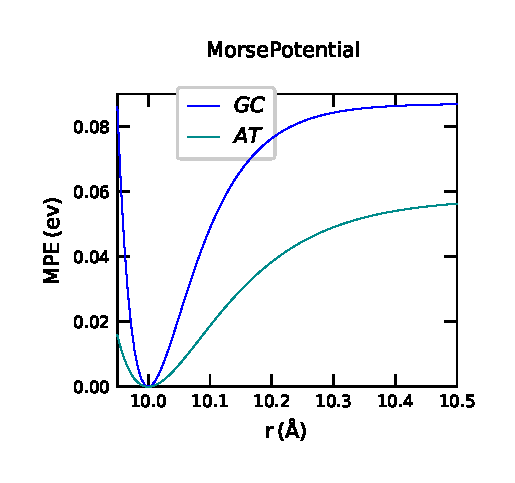
\includegraphics[width=0.5\textwidth]{Morse_Potential_GC_AT.eps}
  \floatsetup[figure]{font=1}
  \caption{\small Morse potential for AT and GC base pairs. This figure compares range and depth of morse potential for AT and GC base pairs for depth $D_{AT}=0.058$ and $D_{GC}=1.5\times D_{AT}$ and for range $a_{AT}=8.5\angstrom^{-1} $ and $a_{GC}=13.8\angstrom^{-1}$\,.}
\label{fig:Morse Potential}
\end{figure}
%
\newpage
\subsection{Stacking interaction between adjacent base pairs}
%
  \begin{equation} \label{stacking}
    U_s(r_n,r_{n-1}) = \frac{S}{2}
    \left(1 + \rho \, e^{-b_s \, \left(r_n + r_{n-1} - 2 R_0\right)} \right) \left(r_n - r_{n-1} \right)^2 \, \, .  
  \end{equation}
  %
  The harmonic interaction with coupling constant $S$ between the radial distances $r_n$ and
  $r_{n-1}$ opposes sliding motion of one base pair over another. The harmonic coupling is
  multiplied by a term that strengthens the coupling when the molecule is closed and makes
  it weaker when it is open, taking into account the different stiffness of double-stranded DNA
  compared to single-stranded DNA. Moreover, the stacking interaction stabilizes the
  closed B-form DNA with respect to opening of a single base pair and thus makes the
  DNA melting transition more cooperative.\\
%
\subsection{Backbone stretching}
%
  \begin{equation} \label{backbone}
    U_b(l_n) = \frac{B}{2} \left(l_n - L_0 \right)^2
  \end{equation}
  %
  is the elastic potential energy of a backbone segment of length $l_n$
  and equilibrium length $L_0$ where $B$ is the elastic constant for backbone stretching. 
%
\newpage
\subsection{Coupling between helical twist, rise, and base pair opening}
%
  \begin{equation} \label{coupling}
    U_c(r_n,r_{n-1},\theta_n,l_n) = \frac{C}{2} \, e^{-b_c \, (r_n + r_{n-1} - 2 R_0)} \left(h_n - H_0 \right)^2
  \end{equation}   
  %
  where $h_n$ is the distance (rise) between base pair planes $n-1$ and $n$ given by
  \begin{equation} \label{hn}
  h_n = \sqrt{l_n^2 - r_n^2 - r_{n-1}^2 + 2 r_n r_{n-1} \cos(\theta_n)} \, \, \, .
  \end{equation}    
  %
  For later reference we note that for $r_n = r_{n-1}$
  %
  \begin{equation} \label{hnrr}
    h_n = \sqrt{l_n^2 - 2 r_n^2 \, (1 - \cos(\theta_n)} \, \, \, , \quad r_n = r_{n-1} 
  \end{equation}
  %
  and for $\theta_n = \phi_n - \phi_{n-1} = 0$
  \begin{equation} \label{hntheta0}
    h_n = \sqrt{l_n^2 - (r_n - r_{n-1})^2} \, \, \, , \quad \theta_n = 0 \, \, .
  \end{equation}  
  %
  Values of $l_n$, $r_n$, $r_{n-1}$, $\theta_n$ for which the argument of the square root
  in Eq.\,(\ref{hn}) is negative are excluded by imposing $U_c = \infty$ for negative
  arguments. This implies that $h_n$ is bounded by $h_n \in [0, l_n]$. Moreover, 
  we assume that the twist angle $\theta_n$ is bounded by $\theta_n \in [-0.1, 0.7]$ rad,
  allowing for slight overwinding of the helix
  beyond the equilibrium twist angle of B-form DNA,
  $\theta_{eq} = 2 \pi / 10.4 = 0.604$ rad (corresponding to 10.4 base pairs per helical turn),
  and slight underwinding of completely denatured DNA beyond $\theta = 0$.

  The value of $H_0$ in Eq.\,(\ref{coupling}) is chosen such that for closed B-form DNA
  the potential energy $U_c$ results in a helical structure with thermal averages
  $\langle h_n \rangle = 3.4 \, \angstrom$ and $\langle \theta_n \rangle = 2 \pi / 10.4$.
  This is incorporated by choosing
  $L_0 = 6.853 \, \angstrom$ for the equilibrium length of a backbone segment in
  Eq.\,(\ref{backbone}) and $H_0 = 2.9 \, \angstrom$ in Eq.\,(\ref{coupling}).

  The elastic coupling between helical twist, rise, and base pair opening decreases with
  base pair opening, and is absent for completely denatured DNA. This effect is modeled by
  the exponential factor in Eq.\,(\ref{coupling}) so that the elastic coupling
  is exponentially attenuated with a decay length $b_c^{-1}$.
  We choose $b_c^{-1} = 10 \angstrom$ corresponding to the equilibrium radial distance $R_0$
  of a base pair in B-form DNA. The elastic energy $U_c(r,\theta)$ as a function of 
  $r_n = r_{n-1} \equiv r$ and $\theta_n \equiv \theta$ for fixed $l_n = L_0$ is shown in Fig.~
  \ref{fig:h_and_elastic_energy}.
  %
   \begin{figure}[!h]
    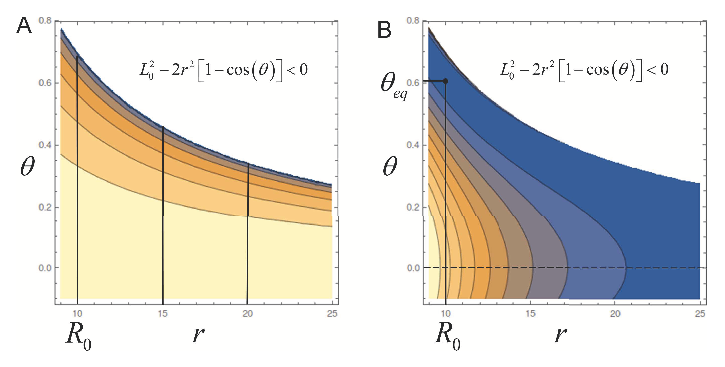
\includegraphics[width=1\textwidth]{h_and_elastic_energy.eps}
    \floatsetup[figure]{font=1}
    \caption{Contour plots of (A) the helical rise $h_n\left(r,\theta\right)$ and (B) corresponding elastic
      energy $U_c\left(r,\theta\right)$ as function of $r_n = r_{n-1} \equiv r$ and $\theta_n \equiv \theta$
      for fixed $l_n = L_0$ (see Eqs.\,(\ref{coupling}) and (\ref{hnrr})).
      The upper right region (shown in white) correspond to negative values of the argument of the
      square root in Eq.\,(\ref{hnrr}) and is excluded.
      (A) shows that for fixed radial distance $r$ (vertical lines) an increasing helical rise $h$
      corresponds to decreasing twist $\theta$, {\em i.e.}, unwinding of the double helix.
      The shape of the minimum of the elastic energy $U_c\left(r,\theta\right)$ in (B) shows that a decreasing
      twist $\theta$, in turn, favors increasing values $r$, {\em i.e.}, opening of base pairs.}
    \label{fig:h_and_elastic_energy}
  
  \end{figure}
%
\newpage
\subsection{External stretching force}
%
  \begin{equation} \label{force}
  U_f(r_n,r_{n-1},\theta_n,l_n) = - f h_n \, \, ,
  \end{equation}
  %
  with the distance $h_n$ between base pair planes $n$ and $n-1$ from Eq.\,(\ref{hn}),
  is the potential energy from applying a stretching force at one end of
  the molecule. Note that Eqs. (\ref{coupling}) and (\ref{force}) result in a coupling
  of helical rise, twist, and base pair opening to the stretching force $f$.
  Since in our model the two bases of a base pair are confined to a plane
  perpendicular to the helical axis, the stretching force $f$ acts on the whole terminal
  base pair simultaneously, corresponding to a force $f/2$ applied to each base of the
  terminal base pair. 
  There is no torsional constraint, i.e., the terminal base pair is free to rotate
  about the helical axis. Eqs.\,(\ref{coupling}), (\ref{hn}) and (\ref{force}) result in a coupling of helical rise,
  twist, and base pair opening to the stretching force $f$. To understand the reason for this
  coupling, Fig.~\ref{fig:h_and_elastic_energy} shows contour plots of the helical rise
  $h_n(r,\theta)$ and the corresponding elastic energy $U_c(r,\theta)$ as functions of
  $r_n = r_{n-1} \equiv r$ and $\theta_n \equiv \theta$ for fixed $l_n = L_0$
  (see Eqs.\,(\ref{coupling}) and (\ref{hnrr})).
  (A) shows that for fixed radial distance $r$ (vertical lines) an increasing helical rise $h$,
  induced by the stretching force $f$, corresponds to decreasing twist $\theta$, {\em i.e.},
  unwinding of the double helix. The shape of the minimum of the elastic energy $U_c(r,\theta)$
  in (B) shows that a decreasing twist $\theta$, in turn, favors increasing values of $r$,
  {\em i.e.}, opening of base pairs. Combining these two effects one obtains that an increasing
  stretching force $f$ favors unwinding of the double helix and opening of base pairs.\\ 
%
\newpage
\begin{table} [!h]
\centering  
\begin{tabular}{ | l | l | l | l |} 
    \hline
    Parameter & Symbol & Value & Unit \\ \hline
    Morse potential inverse range & $a_n$ & $a_{\text{AT}} = 8.4$ & $\angstrom^{-1}$ \\
    & & $a_{\text{GC}} = 13.8$ & \\ \hline
    Morse potential depth & $D_n$ & $D_{\text{AT}} = 0.058$ & eV \\
    & & $D_{\text{GC}} = 1.5 \, D_{\text{AT}}$ & \\ \hline
    Equilibrium radial distance of a base & $R_0$ & 10 & $\angstrom$ \\ \hline
    Threshold radial distance to consider base pair open & $r_d$ & 10.25 & $\angstrom$ \\ \hline
    Backbone segment equilibrium length & $L_0$ & 6.853 & $\angstrom$ \\ \hline
    Backbone stretching elastic constant & $B$ & 0.128 & ev\,$\angstrom^{-2}$ \\ \hline
    Stacking interaction elastic constant & $S$ & 0.1 & ev\,$\angstrom^{-2}$ \\ \hline
    Stacking interaction coupling parameter & $\rho$ & 2 &  \\ \hline
    Stacking interaction inverse range & $b_s$ & 0.7 & $\angstrom^{-1}$ \\ \hline
    Elastic coupling twist, rise, base pair opening & C & 0.028
    & ev\,$\angstrom^{-2}$ \\ \hline 
    Elastic coupling inverse range & $b_{el}$ & 0.1 & $\angstrom^{-1}$ \\ \hline
    Rise per base pair at mechanical equilibrium & $H_0$ & 2.9 & $\angstrom$ \\ \hline
    Energy constant for twist & $c_{tw}$ & 5.64 & $\text{eV}/{\text{rad}^2}$ \\ \hline
    \hline
    \end{tabular}
    \caption{Set of parameters for the potential energy.}
    \label{table_parameters}
    \end{table}
\newpage
%
\section{Monte-Carlo simulations}
Monte Carlo simulation technique is useful to that uses a stochastic method to obtain a new configuration of the system of interest. It is an importance sampling that describes the system at equilibrium. The advantage of the Monte-Carlo method is that it escapes solving Newtons' equations of motion. But the disadvantage is that we miss the dynamical information from it. Monte Carlo simulation calculates equilibrium thermodynamic and physical properties of a system of interest~\cite{earl2008monte}. Let to calculate the average value of some property be $<A>$. For N randomly generated Montecarlo points, in configuration space $r^{N}$ the average value is \begin{equation}
<A>\approx \frac{1}{N_{mc}}\sum\limits_{i=1}^{N_{mc}} A(r_{i}^{N})\,\, .\end{equation}
 
%

\subsection{Monte Carlo simulation procedure}
{\label{MCSP}}
The goal of the Monte Carlo simulation procedure is to obtain the melting curve as a function of temperature for thermal DNA denaturation and as a function of temperature and force for force-induced DNA Dnaturations. We performed three different trial moves base-pair opening move\ref{bopmv}, Twisting move\ref{tmv}, and Stretching move\ref{smv} starting from mechanical equilibrium and obtained average fraction $f$ of open base pairs  from the condition $\langle r_{n} \rangle $ $>$ $r_{open}$, $l$ average fraction of open base pairs obtained from the overall simulation, $n_{b}$ average number of the bubbles formed for overall simulation, $l_{b}$ average size of the bubble formed for overall simulation, $h$ the average rise of base plane distance for overall simulation, and $\theta$ the average twist angle for overall simulation. \\
\indent
We use the standard metropolis Monte Carlo algorithm~\cite{ares2005bubble,earl2008monte} to produce an equilibrium state of the system. We 
initialize base pairs , pick single base-pair $n_0$ at random and draw new value of the variable $r_{n_0}, L_{n_0}$, and $\theta_{n_0}$ from random Gaussian distribution. The energy of the old configuration and new configuration is calculated. If the potential energy of a new configuration is lower than the old configuration, the new configuration is accepted unconditionally. Otherwise new configuration is accepted with Metropolis probability for $U_{trl}$ $>$ $U_{current}$
% 
\begin{equation}\label{mpol}
p = \textrm{min}\left(1,\exp \left[-\left(\frac{U_{trl}-U_{current}}{k_BT} \right)\right] \right)
\end{equation}
%
By averaging over  the properties of the accepted configurations, we obtain the  profile  $\left\langle  r_{n} \right\rangle$, $\left\langle \theta_{n} \right\rangle$ for given sequence of bps n=1,...N by MC simulation; calculate $l$ by applying the condition that at least one base pairs is closed and $f$ by using the criterion that bp n is considered "open"  if $\left\langle r_{n} \right\rangle $ $\geq$ $10.25 \angstrom$. \\
\subsection{Base-pair opening move}{\label{bopmv}}
Without the exponential term, the stacking interaction between radial distances $r_n$, $r_{n-1}$
of bases in neighboring base pair planes reads
%
\begin{equation} \label{stacking2}
    U_s(r_n,r_{n-1}) = \frac{S}{2} \left(r_n - r_{n-1} \right)^2 \, \, .  
\end{equation}
%
The motion of the radial distances $r_n$, $r_{n-1}$ can be described in terms of the variables
%
\begin{equation} \label{xy}
  x = \frac{1}{\sqrt{2}} \left(r_n - r_{n-1}\right) \, \, , \quad
  y = \frac{1}{\sqrt{2}} \left(r_n + r_{n-1}\right) \, \, ,
\end{equation}
%
which represent the out-of-phase and in-phase (center of mass) relative motions of
$r_n$ and $r_{n-1}$, respectively. Writing Eq.\,(\ref{xy}) in matrix form 
$ {x \choose y} = A {r_n \choose r_{n-1}}$ one finds that $\det(A)=1$, i.e., the
determinant of the Jacobian matrix $A$ of the transformation $(r_n, r_{n-1}) \to (x,y)$ is equal
to one. In terms of the variable $x$ Eq.\,(\ref{stacking2}) reads $U_s(x) = S \, x^2$.
The standard deviation $\sigma$ of $x$ in a canonical ensemble with Boltzmann weight
$\exp\left[-\beta U_s(x) \right]$ is given by
%
\begin{equation} \label{sd}
  \sigma = \sqrt{\langle x^2 \rangle} = \sqrt{\frac{k_B T}{2 S}}
\end{equation}
%
where $\beta = 1 / (k_B T)$ and $k_B$ is the Boltzmann constant.
%
Accordingly, for a given current value $r_{cur}$ of the radial displacement $r_n$ a trial value
is chosen according to
%
\begin{equation} \label{rtl}
r_{trl} = r_{cur} + \sqrt{\frac{k_BT}{2S}} \xi
\end{equation}
%
where $\xi$ is a standard Gaussian random variable with $\langle \xi \rangle = 0$ and
$\langle \xi^2 \rangle = 1$. With this choice the variance of base-pair opening moves
corresponds to the variance of thermal fluctuations of $x$, i.e.,
%
\begin{equation} \label{var} 
  \langle \left(r_{trl} - r_{cur} \right)^2 \rangle = \frac{k_{B}T}{2S} \langle \xi^2 \rangle =
  \frac{k_{B}T}{2S} = \sigma^2 \, \, .
\end{equation}\\


\subsection{Twisting move}{\label{tmv}}
%
\begin{equation}\label{twe}
 U_{tw} = 2 \pi^2 \frac{K}{H_{0}} \left(\Delta T_{w} \right)^2 \, \,
\end{equation} 
%
is the potential energy for twisting. 
\begin{equation}\label{twe}
\Delta T_{w} = \frac{1}{2\pi} \left(\theta_{n}-\theta_{0} \right) \, \,
\end{equation}
%
is the angular displacement.
%
\begin{equation}\label{ctwe}
U_{tw}= \frac{1}{2} c_{tw} \left(\theta_{n}-\theta_{0} \right)^2 \, \, 
\end{equation}
%
is the form of twisting energy.
%
\begin{equation}\label{twc}
c_{tw} = \frac{K}{H_{0}} = 5.64 \frac{ev}{rad^2} \,\,
\end{equation}
%
is the twisting constant obtained from the twist modulus equivalent to  $2.61 \times 10^{-19}$ erg cm per rad. and $\theta_n = \left(\phi_n-\phi_{n-1} \right) $ is angle of twist. The standard deviation $\sigma$ of $\theta$ in a canonical ensemble with Boltzmann weight
$\exp \left[-\beta U_{tw} \left(\theta_n-\theta_0 \right) \right]$ is given by, 
%
\begin{equation}\label{tsd}
\sigma = \sqrt{\frac{1}{c_{tw} \beta}} \, \,
\end{equation}
%
where $\beta = 1 / (k_B T)$ and $k_B$ is the Boltzmann constant.
%
Accordingly, for a given current value $\theta_{cur}$ of the angular displacement $\theta_n$ a trial value
is chosen according to
%
\begin{equation} \label{thetatrl}
\theta_{trl} = \theta_{cur} + \sqrt{\frac{k_BT}{c_{tw}}} \xi
\end{equation}
%
where $\xi$ is a standard Gaussian random variable with $\langle \xi \rangle = 0$ and
$\langle \xi^2 \rangle = 1$. With this choice the variance of Twisting moves
corresponds to the variance of thermal fluctuations of $\left(\theta_n-\theta_0 \right)$, i.e.,
%
\begin{equation} \label{tvar} 
  \left< \left(\theta_{trl} - \theta_{cur} \right)^2 \right> = \frac{k_{B}T}{c_{tw}} \langle \xi^2 \rangle =
  \frac{k_{B}T}{c_{tw}} = \sigma^2 \, \, .
\end{equation}
%
\subsection{Stretching move} {\label{smv}}
\begin{equation}\label{stm}
U_b = \frac{1}{2} B \left(l_n-l_{0}\right)^2
\end{equation}
%
 is the potential for backbone stretching.
%
\begin{equation}\label{bc}
B=\frac{K_{modu}}{H_{0}} = 0.128 eV/\angstrom^2
\end{equation}
%  
is the stretching constant obtained from the stretching modulus equivalent to 594pN per helical rise $H_{0}$. The standard deviation $\sigma$ of $l$ in a canonical ensemble with Boltzmann weight
$\exp\left[-\beta U_b\left(l_n-l_0\right) \right]$ is given by
%
\begin{equation} \label{ssd}
  \sigma = \sqrt{\frac{k_B T}{B}}
\end{equation}
%
where $\beta = 1 / (k_B T)$ and $k_B$ is the Boltzmann constant.
%
Accordingly, for a given current value $l_{cur}$ of the back bone displacement $l_n$ a trial value
is chosen according to
%
\begin{equation} \label{ltrl}
l_{trl} = l_{cur} + \sqrt{\frac{k_BT}{B}} \xi
\end{equation}
%
where $\xi$ is a standard Gaussian random variable with $\langle \xi \rangle = 0$ and
$\langle \xi^2 \rangle = 1$. With this choice the variance of stretching moves
corresponds to the variance of thermal fluctuations of $l$, i.e.,
%
\begin{equation} \label{lvar} 
  \left< \left(l_{trl} - l_{cur} \right)^2 \right> = \frac{k_{B}T}{B} \left< \xi^2 \right> =
  \frac{k_{B}T}{B} = \sigma^2 \, \, .
\end{equation}
%
\newpage
\section{Double-stranded ensemble}
{\label{dse}}
T.S. Van Erp~\cite{van2006bubbles} suggested that in the thermodynamic limit of an infinite DNA chain, the use of full NVT or NVE ensemble is significant, but the finite DNA chain like PBD model have not much meaning. So we required to define a special ensemble called DNA ensemble to address these issues. PBD model comprises a single chain in infinite solution because of which dsDNA is free to go to large separation due to a plateau of the Morse potential. But in an experiment consisting undiluted solution, due to hybridization two-strand come closer to pair with the complementary strand. Thus, for a finite concentration, the experimental result cannot be reproduced using equilibrium statistics in the full phase space. Therefore, there required an MD or Monte Carlo simulations which begins from certain initial configuration to confine the phase space. A configuration $\lbrace r_{n}\rbrace$ a dsDNA molecules such that $r_{n} < r_{open}$ for at least one $n \in \left[1:N \right]$ where $r_{open}$ the opening threshold definition. A configuration is completely denatured if $r_{n} > r_{open}$ for all n. Thus, dsDNA is defined as all configuration assigned as dsDNA together with their corresponding Boltzmann weight. If $R \left(r^N \right)$ be any function, then the statistical average in the full phase space is defined as,
% 
\begin{equation}\label{ssav}
\left< R \right> \equiv \frac{\int dr^N R \left(r^N\right) \exp{\left[  -\beta U \right] } } {\int dr^N \exp{\left[-\beta U \right]}}
\end{equation}
%
with $dr^N \equiv dr_{N}, dr_{n-1}...dr_{1}$. The exponential term represents the probability distribution density with Boltzmann factor $\beta$. Using weight function $\mu \left(r^N \right)$ the ensemble average of $R\left(r^N\right)$ in dsDNAE can be expressed as weighted average as shown below,
%
\begin{equation}
\left< R \left( r^N \right) \right>_{\mu} \equiv \frac{\left< R \left( r^N \right)_{\mu} \right>}{\left< \mu \right>}
\end{equation}
%
\begin{equation}\label{wf}
\mu\equiv 1- \Pi_{k=1}^N\eta_{n}
\end{equation}
%
where $\eta_{n}$ is the Heaviside step function whose value is 1 for open base pair and 0 otherwise. The value of $\mu$ is 1 for at least one base pair is not open and 0 for when all base pairs are opened. The use of dsDNAE not only removes the problems of non-normalizability of the full phase space equilibrium distribution but also represents the actual experimental situations at a temperature below the denaturation transition.
%
\newpage
\chapter{Result and Discussion}
Since DNA denaturations are Ising Type \,i.e, opening, and closing of base pairs~\cite{poland1966d}. We applied Monte Carlo simulations technique to study such behavior of DNA helicoids. We chose 100 DNA molecules for thermal denaturations and 200 molecules for force-induced DNA denaturations. We studied the denaturations behavior of the  Bound DNA sequence of length as shown in Table~\ref{table_length_sequence}.The first three sequences of the table were used to study the thermal denaturations behavior whereas the remaining three gave the appropriate informaitons about the force-induced DNA denaturations. We define the parameters as shown in table \,\ref{table_parameters}. The parameters of the morse potential are base pair dependent so that their values are different for AT and GC base pairs. In the simulations '0' represent the AT base pairs and '1' represent the GC base pairs. Thermal denaturations occur as a function of temperature whereas Force-induced denaturations occur as a function of force at room temperature. With the help of randomly generated numbers, we picked random base-pair $n_{0}$ . Since our DNA model has three degrees of freedom, we made three different trial moves for base-pair $n_0$. Using uniform random number we allocated the 40percent of the move for open base pairs, between 40 percent to 80 percent of the move for twisting, and remaining 20 percent for the stretching move. Our simulations started from thermal-mechanical equilibrium. The equilibrium values are shown in Table~\ref{table_parameters}. For each temperature and force, we run a simulation, for each simulation $10^6$ steps were used for thermalization, after thermalization $10^4$ MC steps were used as a saved configuration, for each saved configuration $10^2$ MC steps were performed. Periodic boundary conditions were chosen to avoid a large number of the denaturations at the end. We compared our Monte Carlo simulations results with the experimental result given at the paper~\cite{zeng2003length,zeng2004bubble} which calibrates our DNA models. After calibration, we use the parameters to study the force-induced DNA denaturations phenomenon for the DNA sequence L30B12, L20B8, and L12B6 and we compared the results of our simulations with the experimental results of Strunz et al. , Gaub et al., and Pop et al.~\cite{Strunz:1999, Pope:2001, Morfill:2007}.\\ 
%
\begin{table} [!h]
\centering  
\begin{tabular}{ | l | l |} 
    \hline
    Length & Bubble in-the middle sequence \\ \hline
    L60B36 &\makecell{CCGCCAGCGGCGTTATTACATTTAATTCTTA\\
    AGTATTATAAGTAATATGGCCGCTGCGCC}  \\ \hline
    L42B18 & \makecell{CCGCCAGCGGCGTTAATACTTAAGTATTATG\\
    GCCGCTGCGCC} \\ \hline
    L33B9  &\makecell{CCGCCAGCGGCCTTTACTAAAGGCCGCTGC\\
    GCC}  \\ \hline
    L30B12 &GGCTCCCTTCTACCACTGACATCGCAACGG  \\ \hline
    L20B9  &CGTTGGTGCGGATATCTCGG \\ \hline
    L12B6  &CGCAAAAAAGCG \\ \hline
    \hline
    \end{tabular}
    \caption{Length of DNA sequence\,.}
    \label{table_length_sequence}
    \end{table}
%
\section{Thermal DNA denaturations}
As discussed in Subsec.\,\ref{MCSP}, we have used the standard Metropolis algorithm to perform the Monte Carlo simulations on our helicoidal DNA model. For the simulations, we set minimum and maximum temperature as $30^\circ$  and $100^\circ C$ respectively because at a temperature lower than $30^\circ C$ dsDNA is bounded where as at around $100^\circ C$ we believed all the molecules are completely denatured. For each temperature, we performed a number of simulations. In each of these simulations, we compute the mean profile $\left< r_{n} \right>$, $\left< \theta_{n} \right>$, and $\left< h_{n}\right>$ from which we obtain the fraction of open base pairs and coupling between the helical rise and angle of twist. We consider  the nth base pair to be open if $\left< r_{n} \right>$ exceeds certain threshold $r_{open}$. We calculate the fraction of open base pairs one obtained from the partially opened DNA molecules for overall simulations $l$ and the other $f$ from the saved configurations which satisfies$\left< r_{n} \right>$ $>$ $r_{open}$ for overall simulations. We also calculate the mean number of a bubble formed $n_{b}$ and the mean number of the bubble size $l_b$ for the overall simulations. We compare our results for Bubble-in-the-middle sequences L60B36, L42B18, and L33B9 with the experimental results of the ~\cite{zeng2003length,zeng2004bubble} in the following subsection.
\newpage
\subsection{L60B36}

In Fig.\,\ref{fig:L60b36cal} we present our simulation result for the bubble-in-the-middle sequence L60B36 and compared it with the thermal experimental result of Zeng et al \cite{zeng2003length,zeng2004bubble}\ref{fig:L60B36exp}.The Fig.\,\ref{fig:L60B36exp} is the experimental melting curves and the average fractional length of the bubble $\left< l \right> $. The open circle is the fraction of the open bases which represent the UV absorption data. $p$ represents the fraction of denatured molecules, but in our Monte Carlo simulation result, we ignore the calculation of $p$ because for the long DNA sequences $f=p$. $f$ is normalized to one so that at the end of transition $f=p=1$. The experimental result of Fig.~\ref{fig:L60B36exp} shows that there exist a plateau for $\left< l \right> $ $\approx 0.6$, which is the relative length of the AT-rich region $36/60=0.6$. But our simulation result ignores the possibility of the existence of the plateau because for the finite DNA, the transition is continuous and the bubbles are the diverging size. The experimental data shows that there exists a melting temperature $T_{m}$ at around $62^\circ C$, our simulations show that such temperature exists at around $68^\circ C$. But similar Monte Carlo result like ours was conducted by ~\cite{ares2005bubble} and showed that there exists a plateau at the relative length of AT-rich region at around $65^\circ C$  which is equivalent to the data of long $\lambda$-DNA. From the Fig.~\ref{fig:L60B36lf} we see that fraction of open base pairs $l$ obtained from the partially opened DNA strand and $f$  the fraction of open base pairs obtained from $\left< r_{n} \right> $ $> r_{d}$ are dependent upon the average number of open base pairs and average bubble size. $f$ is normalized to 1 such that bubble denatured to form single-stranded DNA. Fig.~\ref{fig:L60B36bub} shows that bubbles are continuously formed and reach to the maximum at around $60^\circ C$ after that average bubble size $l_b$ increases decreasing average number of bubble which indicates base pairs are opened. Fig.~\ref{fig:L60B36htheta} shows that there exists strong coupling betweening helical rise and twist in the low temperature region below $60^\circ C$, after that the decrease in the value of twist favors the increase in the helical rise i.e, base pair opening.
%
\newpage
\begin{figure}[!h]
        \begin{subfigure}[b]{0.49\textwidth}
                \centering
                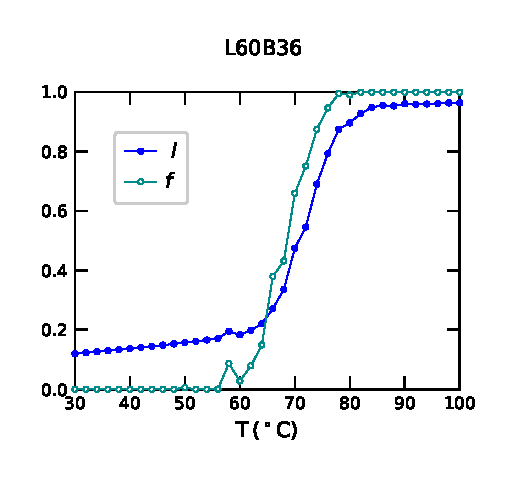
\includegraphics[height=1.9in, width=.8\textwidth]{L60B36_temp_lf.eps}
                \caption{}
                \label{fig:L60B36lf}
        \end{subfigure}%
        \hspace{3pt}
        \begin{subfigure}[b]{0.49\textwidth}
                \centering
                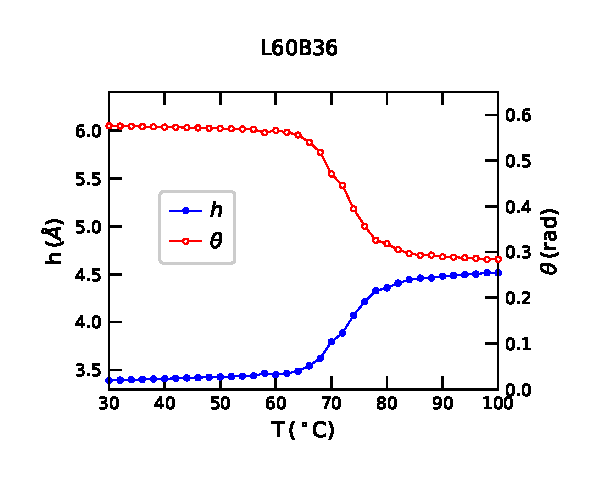
\includegraphics[height=1.9in, width=.8\textwidth]{L60B36_temp_h_theta.eps}
                \caption{}
                \label{fig:L60B36htheta}
        \end{subfigure}%
        
        \begin{subfigure}[b]{0.49\textwidth}
                \centering
                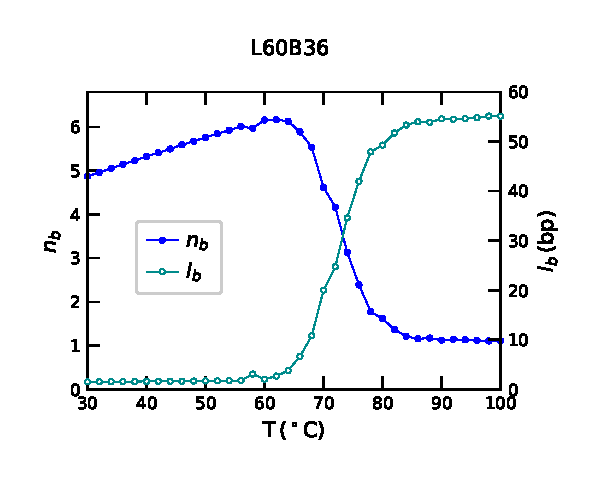
\includegraphics[height=1.9in, width=.8\textwidth]{L60B36_temp_bub.eps}
                \caption{}
                \label{fig:L60B36bub}
        \end{subfigure}%
        \begin{subfigure}[b]{0.49\textwidth}
                \centering
                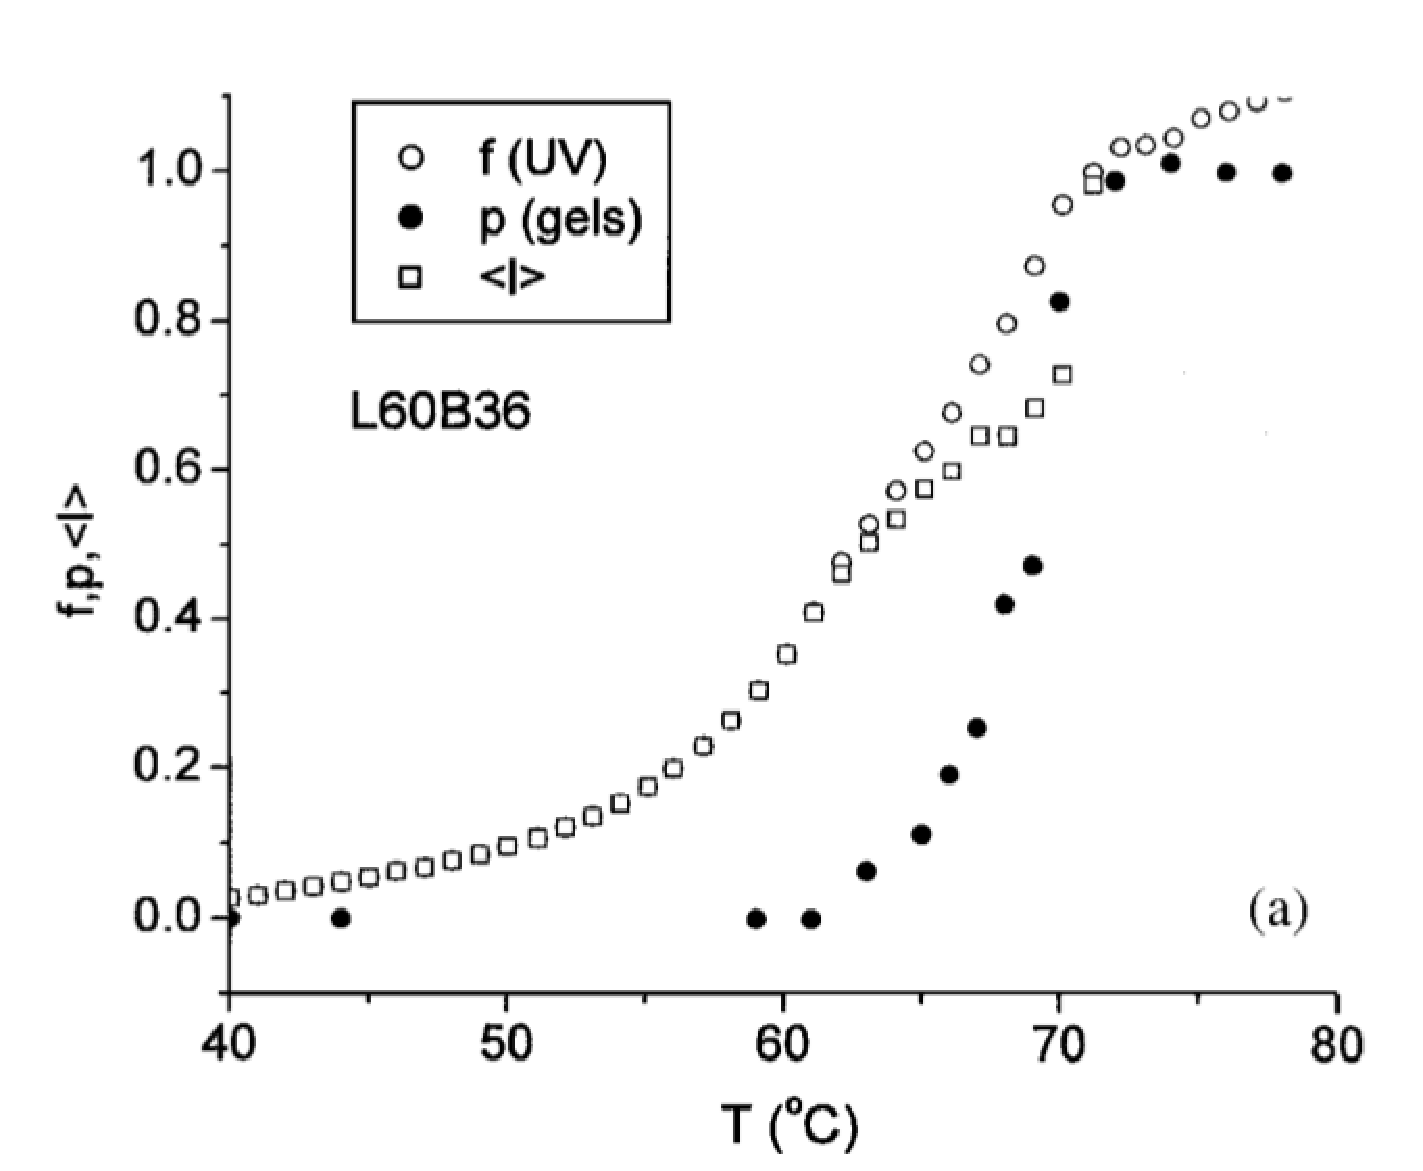
\includegraphics[height=1.9in, width=.8\textwidth]{exp_L60B36.eps}
                \caption{}
                \label{fig:L60B36exp}
        \end{subfigure}%
       
       
\floatsetup[figure]{font=1}
\caption{Thermal melting profile of L60B18 for $d_{AT}=0.058 eV$ and $d_{GC}=1.5*d_{AT}$. Fig(a) represents the plot of the fraction of open base pairs vs temperature. Fig(b) Plot of coupling between the helical rise and twisting versus temperature. Fig(c) gives information about the generation and growth of the bubbles as a function of the temperature. Fig(d) represents the melting profile for L60B36 obtained from the experiment\protect\cite{zeng2003length}\,. } 
\label{fig:L60b36cal}    

\end{figure}
% 
\newpage
\subsection{L42B18}
%
The experimental study of L42B18 shows that at around $68^\circ C$ half of the DNA molecules get thermally denaturated Fig.~\ref{fig:L42B18exp}. But our simulation result Fig.~\ref{fig:L42B18lf} shows that $T_{m}$ exists at around $85^\circ C$  whereas Ares et al showed that such temperature exists at $72^\circ$ Celsius. Experimental result Fig.~\ref{fig:L42B18exp} showed that the plateau exist at  the relative length of AT region 0.42, but  $f$ $\neq$ $\left< l \right>$. Even though bubble formation begins at low temperature, but it did not achieve full size till $85^\circ C$  then after the denaturation begins and bubble generation decreases i.e, basepairs opening. Ares et al~\cite{ares2005bubble} also claim the existence of plateau for such a DNA sequence, but our result denies a such possibility. Our result shows that $f$ still normalize to one but $l$ is deviating from $f$ indicating complete denaturations is still possible in such a temperature range for such sequence but denatrautions phenomenon are less coperative. Fig.~\ref{fig:L42B18htheta} shows that the decrease in the value of the $\theta $ is relatively slower with slow helical rise. Indicating that base pair opening process is relatively slow for such sequence than that of the L60B36 in the given temperature range. 
\newpage
%
\begin{figure}[!h]
        \begin{subfigure}[b]{0.49\textwidth}
                \centering
                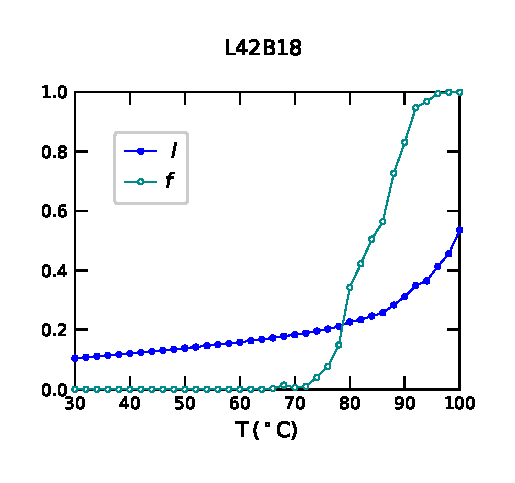
\includegraphics[height=1.9in, width=.8\textwidth]{L42B18_temp_lf.eps}
                \caption{}
                \label{fig:L42B18lf}
        \end{subfigure}%
        \hspace{3pt}
        \begin{subfigure}[b]{0.49\textwidth}
                \centering
                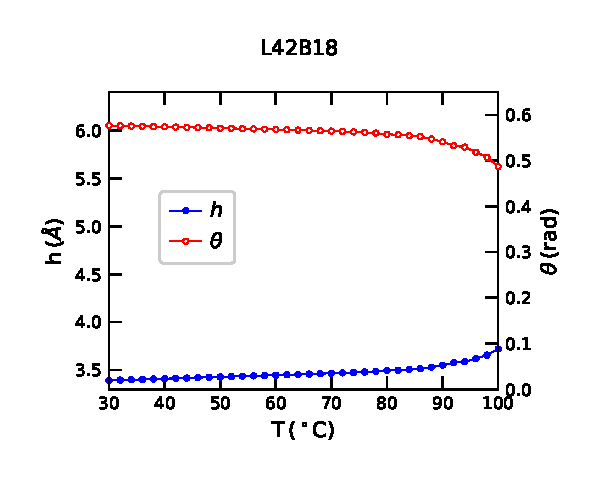
\includegraphics[height=1.9in, width=.8\textwidth]{L42B18_temp_h_theta.eps}
                \caption{}
                \label{fig:L42B18htheta}
        \end{subfigure}%
        
        \begin{subfigure}[b]{0.49\textwidth}
                \centering
                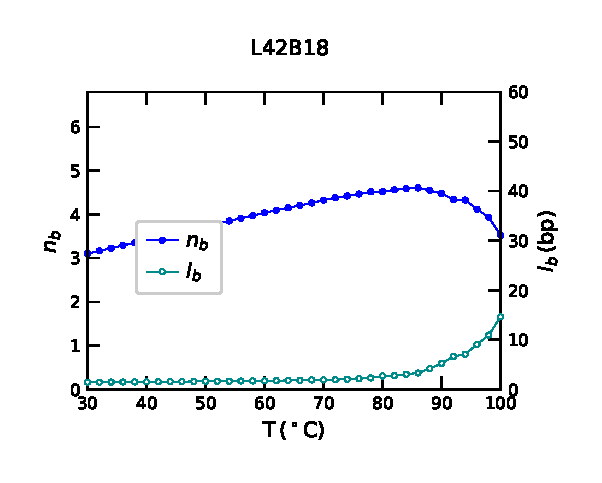
\includegraphics[height=1.9in, width=.8\textwidth]{L42B18_temp_bub.eps}
                \caption{}
                \label{fig:L42B18bub}
        \end{subfigure}%
        \begin{subfigure}[b]{0.49\textwidth}
                \centering
                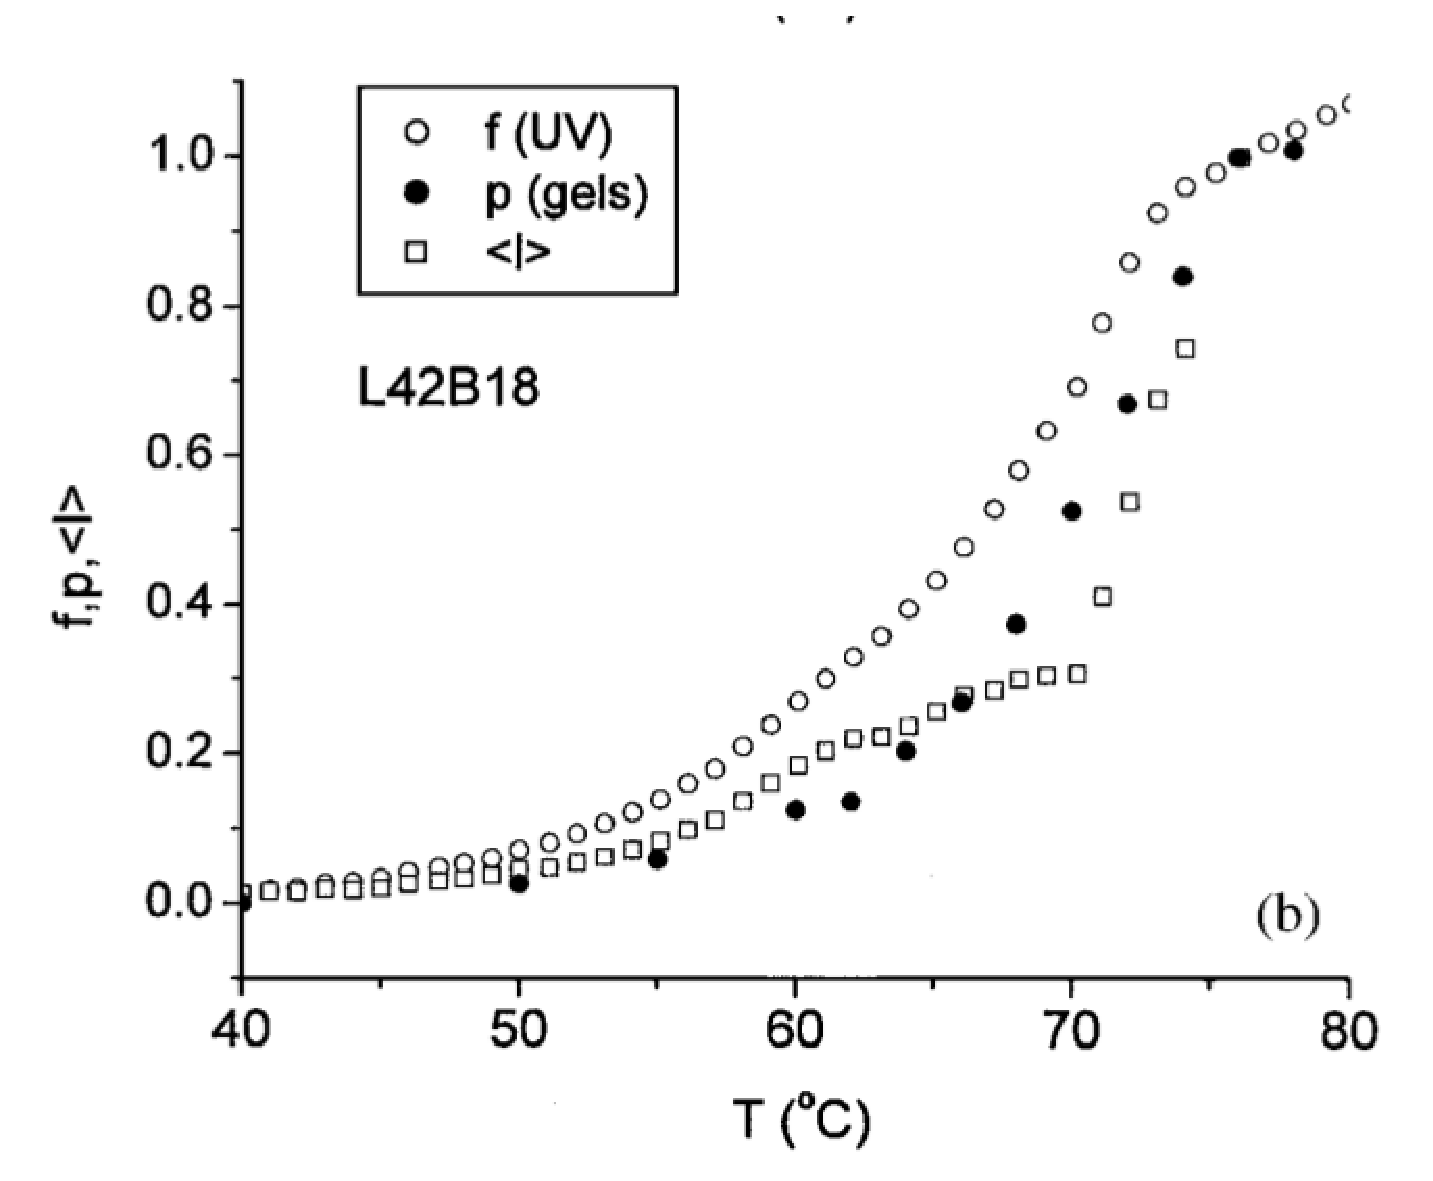
\includegraphics[height=1.9in, width=.8\textwidth]{exp_L42B18.eps}
                \caption{}
                \label{fig:L42B18exp}
        \end{subfigure}%
       
       
\floatsetup[figure]{font=1}
\caption{Thermal melting profile of L42B18 for $d_{AT}=0.058 eV$ and $d_{GC}=1.5*d_{AT}$. Fig(a) represents the plot of the fraction of open base pairs vs temperature. Fig(b) Plot of coupling between the helical rise and twisting versus temperature. Fig(c) gives information about the generation and growth of the bubbles as a function of the temperature. Fig(d) is the melting profile for L42B18  obtained from experiment~\protect\cite{zeng2003length}\,.} 
\label{fig:L42b18cal}    

\end{figure}
%
\newpage
\subsection{L33B9}
The experimental results of the zing et al~\cite{zeng2003length,zeng2004bubble}\ref{fig:L33B9exp} shows that the melting temperature for short DNA sequence L33B9  exist at around $72^\circ C$ whereas simulation result of~\cite{ares2005bubble} indicates that such temperature exist at around $75^\circ C$. But our simulations show that the proper melting temperature of the such DNA sequence exists at around $95^\circ C$. The experimental result also supports the existence of plateau at the relative length 0.27 of the AT base pair region. Ares et al.~\cite{ares2005bubble} also showed that such plateau is obvious for L33B9. But our result denies the existence of such a plateau region because the DNA denaturation of such sequence is largely continuous and our DNA strand is finite and very short. Our simulaiton results Fig.~\ref{fig:L33B9lf},\ref{fig:L33B9htheta}, and \ref{fig:L33B9bub} show that melting temperature is close to $100^\circ C$, with no complete denaturations of the molecules. The denaturation phenomenon is higly non-cooperative.
\newpage
%
\begin{figure}[!h]
        \begin{subfigure}[b]{0.49\textwidth}
                \centering
                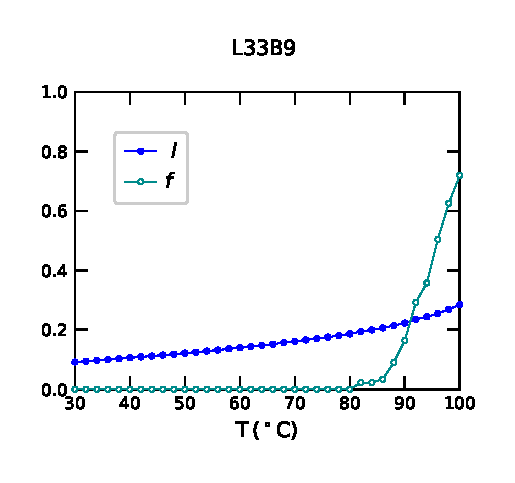
\includegraphics[height=1.9in, width=.8\textwidth]{L33B9_temp_lf.eps}
                \caption{}
                \label{fig:L33B9lf}
        \end{subfigure}%
        \hspace{3pt}
        \begin{subfigure}[b]{0.49\textwidth}
                \centering
                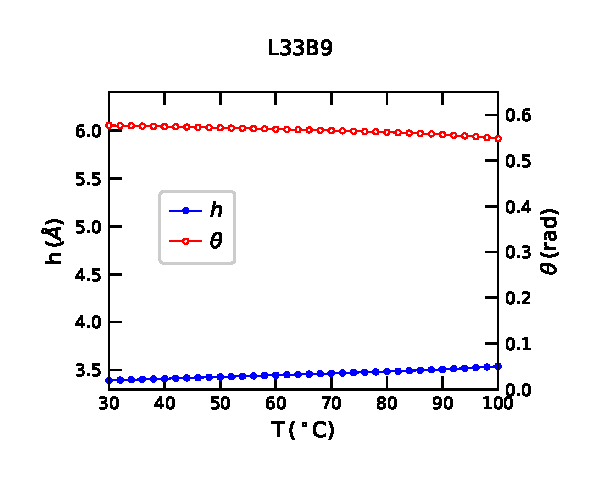
\includegraphics[height=1.9in, width=.8\textwidth]{L33B9_temp_h_theta.eps}
                \caption{}
                \label{fig:L33B9htheta}
        \end{subfigure}%
        
        \begin{subfigure}[b]{0.49\textwidth}
                \centering
                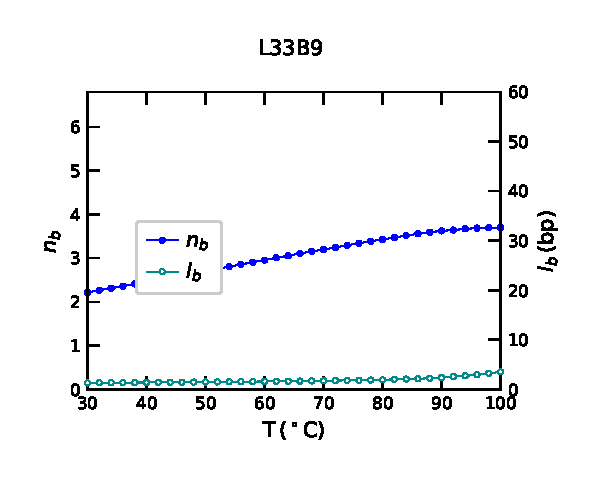
\includegraphics[height=1.9in, width=.8\textwidth]{L33B9_temp_bub.eps}
                \caption{}
                \label{fig:L33B9bub}
        \end{subfigure}%
        \begin{subfigure}[b]{0.49\textwidth}
                \centering
                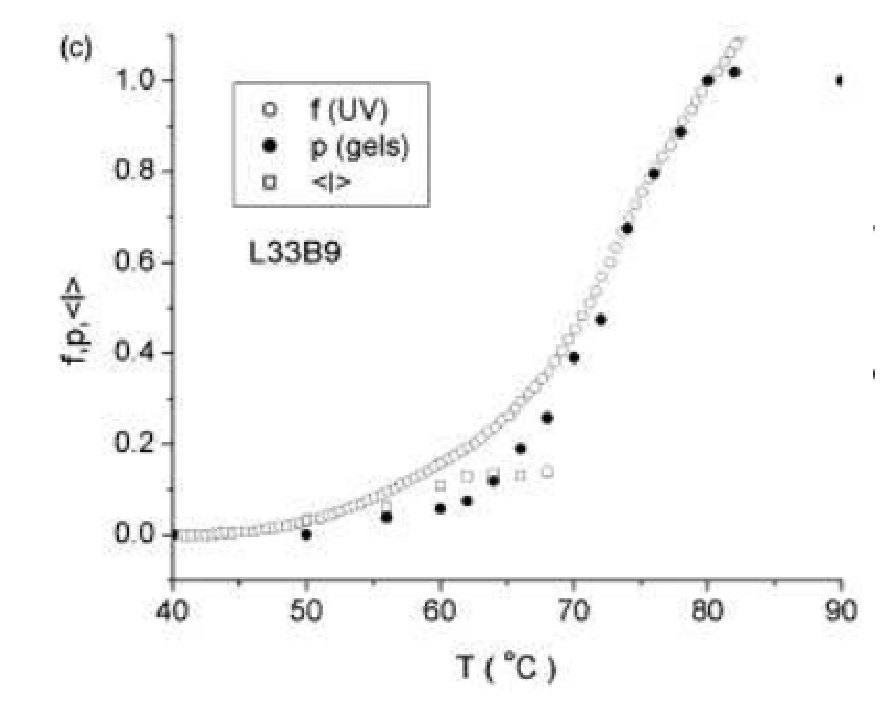
\includegraphics[height=1.9in, width=.8\textwidth]{exp_L33B9.eps}
                \caption{}
                \label{fig:L33B9exp}
        \end{subfigure}%
       
       
\floatsetup[figure]{font=1}
\caption{Thermal melting profile of L33B9 for $d_{AT}=0.058 eV$ and $d_{GC}=1.5*d_{AT}$. Fig(a) represents the plot of the fraction of open base pairs vs temperature. Fig(b) Plot of coupling between the helical rise and twisting versus temperature. Fig(c) gives information about the generation and growth of the bubbles as a function of the temperature. Fig(d) is the melting profile for  L33B9 obtained from the experiment~\protect\cite{zeng2004bubble}\,. } 
\label{fig:L33b9cal}    

\end{figure}
%
\newpage
\section{Force-induced DNA denaturations}
\subsection{L30B12}
  Under Physiological conditions Strunz et al and his team~\cite{Strunz:1999} researched on  DNA duplex with base pairs  30 to measure the mechanical forces required to separate a single DNA duplex. The opposite 5' -ends were pulled as a function of the loading rate. They found that unbinding forces depend on the loading rates and ranges from 20 to 50$pN$. The data obtained from this single molecular result can be compared with our data obtained from simulations. The DNA oligomer d(GGCTCCCTTCTACCACTGACATCGCAACGG) which contains 30 bases were chosen. Complementary oligonucleotides were covalently fixed on the tip of an AFM cantilever and a substrate. Unspecific forces between the tip and substrates were removed using polyethylene glycol. The data obtained from the experiment were plotted to obtain the histogram. The pick of the histogram determines the values of the rupture forces. Fig.2 of the paper Strunz et al~\cite{Strunz:1999} shows the probability distributions of the unbinding forces of the last rupture events for 500 $approach/retract cycles$ for a retract velocity of 100$nm/s$. The histograms show that the most probable unbinding force is close to 50$pN$. The result of the Gaussian fitting demonstrates that the rupture force is at around $48\pm2 $ $pN$. The force-displacement curve of Fig.~\ref{fig:L30B12exp} of Strunz et al.~\cite{Strunz:1999} suggests that the last unbinding event occurs at the around 50 pN. We performed the Monte Carlo simulation on DNA30s for the force range 20$pN$ to 60$pN$ at room temperature and obtained the plot as shown in Fig. \ref{fig:L30B12}. Fig.\ref{fig:L30B12lf} is the plot of the fraction of the open base pairs vs force. $l$ indicates the average fraction of the open base-pair obtained from the overall simulation. $f$ is the fraction of the open base pairs satisfying $\left<r_{n}\right> > r_{open}$. The plot indicates that the base pairs are bound up to the force 22$pN$ and stretched elastically till the force reached to the 35$pN$ at which half of the BDNA is denatured to ssDNA. After this force, there begins a non-linear region until the force reaches to around 48$pN$. After this force, the double-stranded DNA is completely unbounded and converted into ssDNA.Fig.~\ref{fig:L30B12extension} shows that the twist angle and helical rise were coupled at force less than 35$pN$ but after this they were decoupled leading dsDNA to ssDNA. The Fig.~\ref{fig:L30B12bub} shows that bubbles were formed  at low force, but it require higher force to get some shape. At around 28$pN$ maximum number of the bubble was formed then after the bubble increases its size whereas bubble generation decrease indicating that the formed bubble started to denature. Fig.~\ref{fig:L30B12extension} shows that about the first $25\%$ of the force-extension curve satisfies the hooks law, about $50\%$ of the curve lies in the nonlinear region and last $25\%$ of the curve lies in the region of unbound.  Our force versus extensions graph well behaves with the result of  Strunz et al.~\cite{Strunz:1999}. As Strunz ~\cite{Strunz:1999}, our result also can predict unbinding events exist at around 50pN. After this force DNA is completely unbound and dsDNA denatured to ssDNA. These plot does not indicate the existence of the B-S transition region because the denaturations completed below the force 65 pN, and  DNA sequences are finite in length.
\newpage
%  
  \begin{figure}[!h]
        \begin{subfigure}[b]{0.49\textwidth}
                \centering
                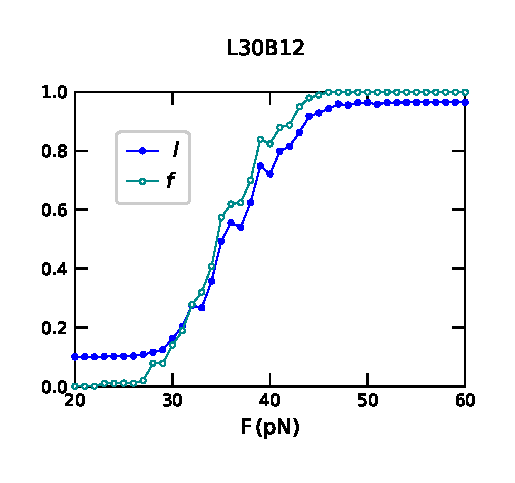
\includegraphics[scale=0.35,height=1.9in, width=.8\textwidth]{L30B12_Strunz_force_lf.eps}
                \caption{}
                \label{fig:L30B12lf}
        \end{subfigure}%
        \hspace{-0.5cm}
        \begin{subfigure}[b]{0.49\textwidth}
                \centering
                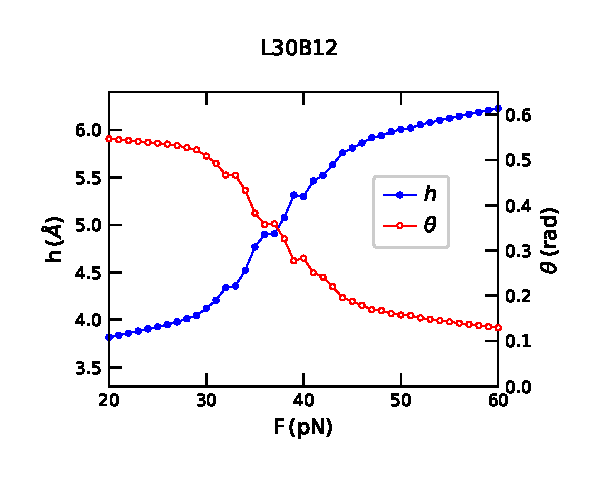
\includegraphics[scale=0.35,height=1.9in, width=.8\textwidth]{L30B12_Strunz_force_h_theta.eps}
                \caption{}
                \label{fig:L30B12htheta}
        \end{subfigure}%
        
        \begin{subfigure}[b]{0.49\textwidth}
                \centering
                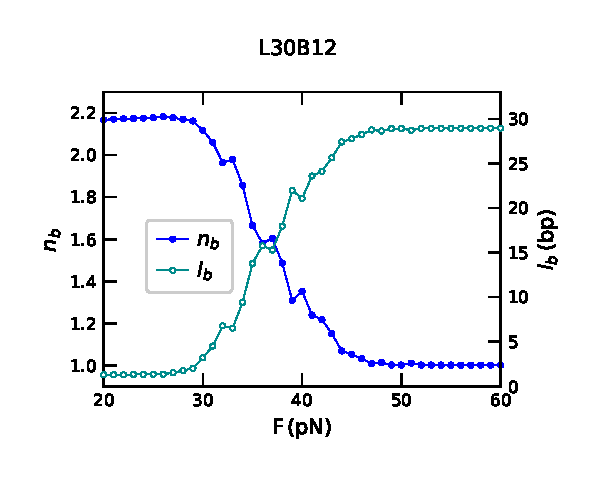
\includegraphics[scale=0.35,height=1.9in, width=.8\textwidth]{L30B12_Strunz_force_bub.eps}
                \caption{}
                \label{fig:L30B12bub}
        \end{subfigure}%
        \hspace{-0.5cm}
        \begin{subfigure}[b]{0.49\textwidth}
                \centering
                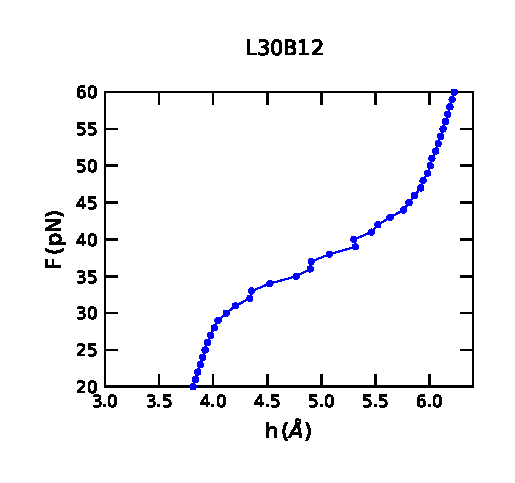
\includegraphics[scale=0.35,height=1.9in, width=.8\textwidth]{L30B12_Strunz_force_extension.eps}
                \caption{}
                \label{fig:L30B12extension}
        \end{subfigure}%
        
        \begin{subfigure}[b]{0.49\textwidth}
                \centering
                \includegraphics[scale=0.35,height=1.9in,width=.8\textwidth]{Strunz_exp.eps}
                \caption{}
                \label{fig:L30B12exp}
        \end{subfigure}%
       
\floatsetup[figure]{font=1}
\caption{\small Melting profile for Force-induced DNA denaturations for DNA sequence L30B12.Fig(a) is the plot of fraction of open base pairs $l$ over all simulations and $f$ the fraction of open base pairs satisfying $\left<r_n\right>$ $>$ $r_{open}$ versus stretching force F. Fig(b) is the plot of helical rise h and twist angle $\theta$ against applied force $F$. Fig(c) is the plot of the average number of a bubble formed  $n_{bub}$ and the average size of bubble $l_b$ against stretching force. Fig~(d) is the plot of stretching force $F$ versus extension. Fig(e) is the plot of the Measurement of unbinding forces obtained from the experimental work of~\protect\cite{Strunz:1999}.The figure displays a force displacement curve in which  two molecules unbind one after the other, the last unbinding event also being at $\approx 50pN$ loading }
\label{fig:L30B12}    

\end{figure}
\newpage
\subsection{L20B8}
%
 Due to experimental noise, Strunz et al. could not observe B-S transition during their measurement of the unbinding forces of short complementary oligonucleotides with 30, 20, and 10 base pairs~\cite{Strunz:1999}. So later Gaub et al. carried out single molecular force spectroscopy experiments with shorts DNA duplex made up of 20 base pairs(DNA20s) and 30 base pairs(DNA30s) with high-resolution cantilevers~\cite{Morfill:2007}. During the experiment, both Complementary DNA strands were covalently immobilized to a cantilever tip and a surface in order to get good data. The application of similar chemistry on both sides (cantilever tip and surface) and the use of PEG as a spacer lower the nonspecific binding events. The force-displacement curve of Fig.~\ref{fig:L20B8exp} taken from the paper Gaub et al~\cite{Morfill:2007} recorded at a retract velocity of 1007$nm/s$ does not show any existence of a B-S transition and dissociates at a force of 53$pN$. Their experimental results show that the majority of the rupture events took place well below the B-S transitions. It is because the used loading rates were not sufficient to reach the melting force of the B-S transition. We performed Monte Carlo simulation for the DNA sequence L20B8s in a force range from 20$pN$ to 80 $pN$ at room temperature. Our simulation results are shown in Fig.~\ref{fig:L20b8}. As Gaub et al. do not observe the plateau during their experiment on DNA20s, our Monte Carlo result also denies the possibility of the formation of the plateau. The value of $l$ and $f$ indicates that the melting force could range from 48$pN$ to 53 $pN$ as shown in Fig.~\ref{fig:L20B8lf}. The Fig.~\ref{fig:L20B8htheta} shows that the bases are coupled till the force reaches 50$pN$, after that the hydrogen bond and staking interaction gets weakened so that the bases are decoupled and the dsDNA denatured to the ss DNA. The number of bubble formation increases linearly up to the force 48$pN$, at which the maximum number of bubbles were formed after that the number of the bubble started to reduce, but the length of the bubbles per base pairs grew. It showed that some of the matured bubble denatured to ssDNA as shown in Fig.~\ref{fig:L20B8bub}. The force-extension curve Fig.~\ref{fig:L20B8extension} at first increases linearly till the forces reach around 50 $pN$ obeying the hooks laws, after that non-linear region beings up to the force equal to  59$pN$ then after dsDNA molecules converted to single-stranded molecules. The comparitive study of force-extension curve of  Fig.~\ref{fig:L20B8extension} and ~\ref{fig:L20B8exp} suggest that our result is in close agreement with the strunz et al. The lack of existence of B-S force plateau both in the experimental result of~\cite{Morfill:2007} and our Monte Carlo result indicates that stretching of short DNA is a non-cooperative process. 
\newpage
%
\begin{figure}[!h]
        \begin{subfigure}[b]{0.49\textwidth}
                \centering
                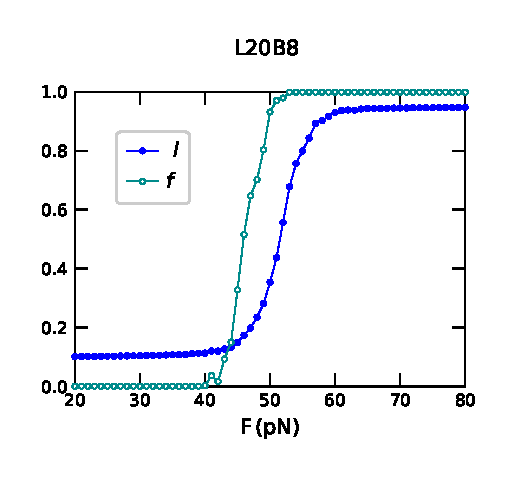
\includegraphics[height=1.9in, width=.8\textwidth]{L20B8_Gaub_force_lf.eps}
                \caption{}
                \label{fig:L20B8lf}
        \end{subfigure}%
        \hspace{1pt}
        \hfill
        \begin{subfigure}[b]{0.49\textwidth}
                \centering
                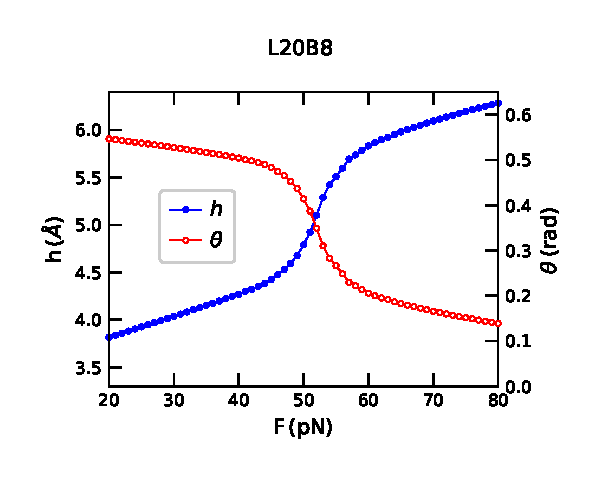
\includegraphics[height=1.9in, width=.8\textwidth]{L20B8_Gaub_force_h_theta.eps}
                \caption{}
                \label{fig:L20B8htheta}
        \end{subfigure}%
        
        \begin{subfigure}[b]{0.49\textwidth}
                \centering
                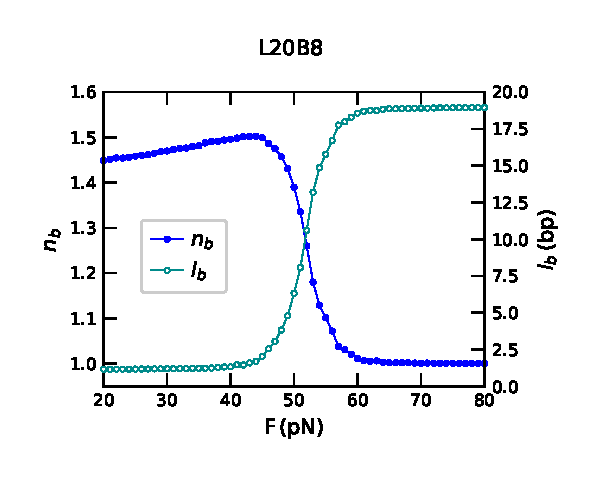
\includegraphics[height=1.9in, width=.8\textwidth]{L20B8_Gaub_force_bub.eps}
                \caption{}
                \label{fig:L20B8bub}
        \end{subfigure}%
        \hspace{1pt}
        \hfill
        \begin{subfigure}[b]{0.49\textwidth}
                \centering
                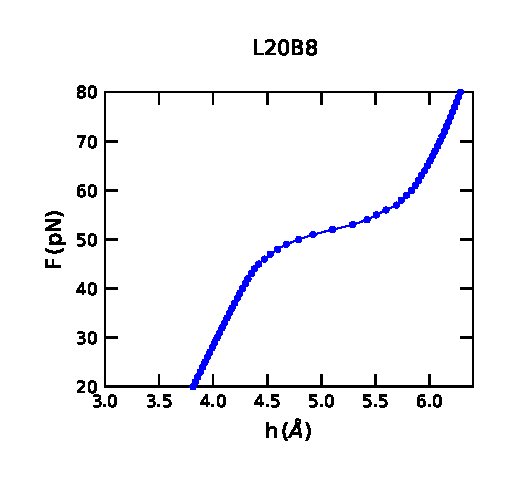
\includegraphics[height=1.9in, width=.8\textwidth]{L20B8_Gaub_force_extension.eps}
                \caption{}
                \label{fig:L20B8extension}
        \end{subfigure}%
        \hspace{1pt}
         \begin{subfigure}[b]{0.49\textwidth}
                \centering
                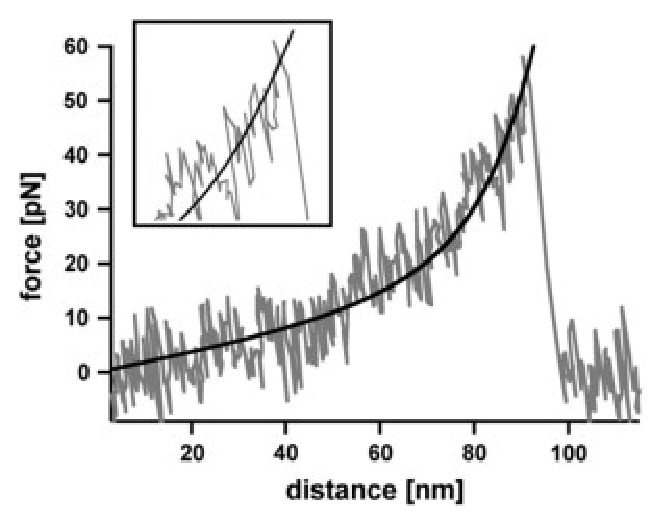
\includegraphics[height=1.9in, width=.8\textwidth]{Extension_Gaub_exp.eps}
                \caption{}
                \label{fig:L20B8exp}
        \end{subfigure}%
       
\floatsetup[figure]{font=1}
\caption{\small Melting profile for Force induced DNA denaturations for DNA sequence L20B8.Fig(a) is the plot of fraction of open base pairs $l$ over all simulations and $f$ the fraction of open base pairs satisfying $\left<r_n\right>$ $>$ $r_{open}$ versus stretching force $F$. Fig(b) is the plot of helical rise $h$ and twist angle $\theta$ against applied force $F$. Fig(c) is the plot of nuber of bubble formed  $n_{bub}$ and size of bubble $l_b$ against stretching force. Fig(d) is the plot of stretching force $F$ versus extension. Fig(e) is the force-extension curve of the 20-basepair DNA duplex(DNA20s);This force-extension curve taken from the paper of~\protect\cite{Morfill:2007} shows a rupture event of a hybridized 20-basepair DNA duplex, recorded at a retract velocity of 1007$nm/s$. The DNA duplexdissociates at a force of 53$pN$, without showing any evidence of the B-S transition(see inset);The froce-extension curve of the  PEG-DNA complex follows the two-state FJC-fit(black) without possessing a measurable deviation.}
\label{fig:L20b8}    

\end{figure}
%
\newpage
\subsection{L12B6}
 Pope and his group~\cite{Pope:2001} studied force-induced melting of a short DNA double helix. For the surface functionalization, they activate the AFM probes and substrate following the technique of \{Noy et al\}. They tethered Single-stranded oligonucleotides of sequence d(CGCAAAAAAGCG) to the gold substrate via hexadecane thiol. Gold-coated probes functionalized with the complementary oligonucleotide d(CGCTTTTTTGCG). To observe the stretching and melting phenomena oligonucleotides were attached through 5' ends. They choose sequence on the basis of an "all-or-none" to get rid off the partial overlap of the constituent single strands. A similar method was adopted to investigate the non-complementary interactions. Force displacement measurements were accomplished using an AFM constructed in the laboratory. Since their system is held under weak force, they consider only rupture force. They maintain their system in a thermally active region so that force-induced melting can be considered as a non-equilibrium process. Therefore, they consider the denaturation forces ranging from 17 to 40$pN$ to separate dsDNA to ssDNA. The rate of loading for each rupture event was determined from the gradient of the force versus the piezo displacement curve at strand separation multiplied by the cantilever retract velocity. The force versus piezo displacement curves of Fig:1a of~\cite{Pope:2001} do not indicate the B-S transitions because their system was at non-equilibrium, DNA strand were too short and were held at a stretching force lower than 65$pN$.
 We performed Monte Carlo simulation for the DNA sequence D12B6 in a force range 40$pN$ to 100$pN$. We begin our simulation keeping our system at mechanical equilibrium, and obtained the plot as shown in Fig.~\ref{fig:L12B6}. Fig.~\ref{fig:L12B6lf} represents the plot of the fraction of open base pairs against the externally applied force. $l$ is the fraction of the open base-pair obtained from the overall simulations average, whereas $f$ is the fraction of open base pair satisfying  $<r_{n}> > r_{open}$. The figure shows that base pairs open even for small forces but it cannot ruptures the molecules until the force reach around 68$pN$. The melting temperature exist at around 75$pN$ where as around 80$pN$ the complete denaturations of the molecules occured. In Fig.~\ref{fig:L12B6htheta}, the decrease in twist angle with increase in helical rise indicates that the basepair opening can occur in low force region, but majority of opening takes place in higher force region. The Fig.~\ref{fig:L12B6bub} reveal that the average number of bubble $n_{b}$ continuously keeping constant size of the bubble. When the force reached around  75$pN$, $n_{b}$ reached to the maximum and then start declining whereas $l_{b}$ started to increasing  suggesting that double-stranded DNA split into single-stranded DNA. The Fig.~\ref{fig:L12B6extension} indicates the extension is longer than L30B12 and L20B8. It reflects that the stress bearing capacity increases with the decrease of the DNA sequence. The comparative study of our result Fig.~\ref{fig:L12B6extension} with the experimental result Fig.~\ref{fig:L12B6exp} of \cite{Pope:2001}  indicates that there does not exist BS transition in short DNA oligomer. As our system was in mechanical equilibrium, we require higher driving forces so that we choose our simulations in the force range 40 to 100$pN$ whereas \cite{Pope:2001} system was thermally active so they only had to apply weak force in the range 17 to 40 $pN$. Our simulations result indicates that short DNA oligonucleotide like D12L6 has a tendency to bear stress than the long DNA molecules.
%
\newpage
\begin{figure}[!h]
        \begin{subfigure}[b]{0.49\textwidth}
                \centering
                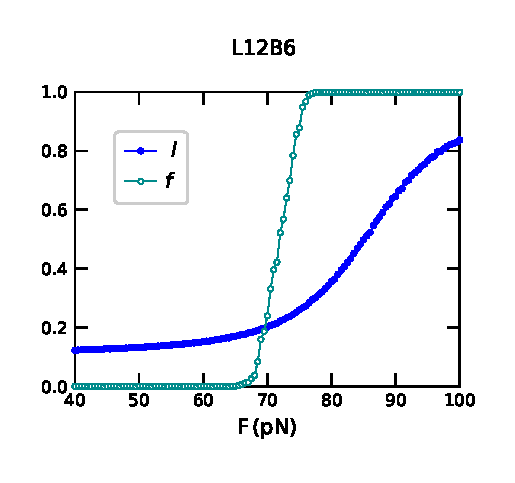
\includegraphics[height=1.9in, width=.8\textwidth]{L12B6_Pope_force_lf.eps}
                \caption{}
                \label{fig:L12B6lf}
        \end{subfigure}%
        \hspace{1pt}
        \hfill
        \begin{subfigure}[b]{0.49\textwidth}
                \centering
                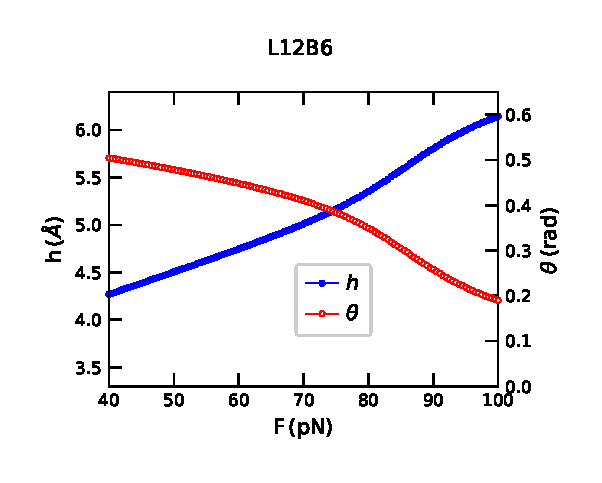
\includegraphics[height=1.9in, width=.8\textwidth]{L12B6_Pope_force_h_theta.eps}
                \caption{}
                \label{fig:L12B6htheta}
        \end{subfigure}%
        
        \begin{subfigure}[b]{0.49\textwidth}
                \centering
                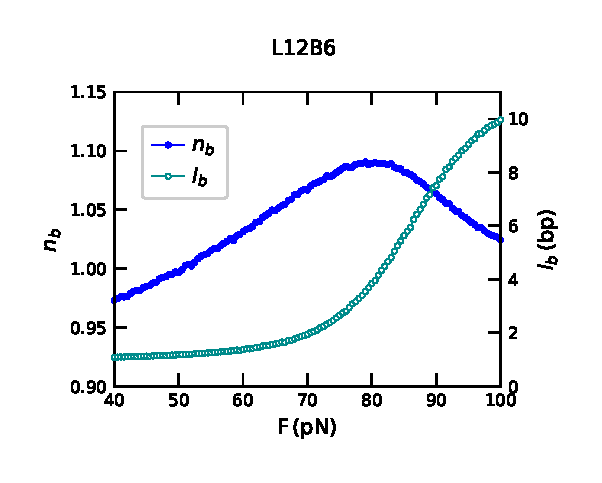
\includegraphics[height=1.9in, width=.8\textwidth]{L12B6_Pope_force_bub.eps}
                \caption{}
                \label{fig:L12B6bub}
        \end{subfigure}%
        \hspace{1pt}
        \hfill
        \begin{subfigure}[b]{0.49\textwidth}
                \centering
                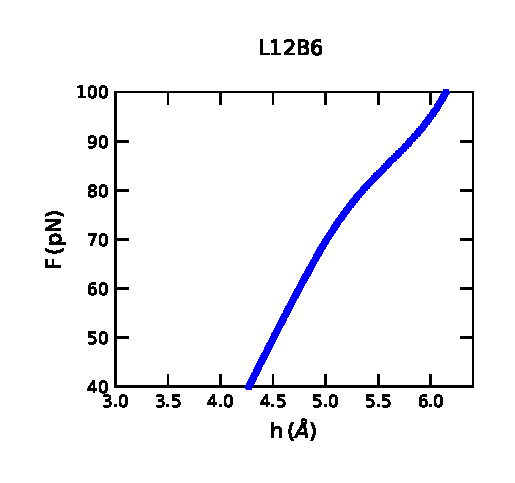
\includegraphics[height=1.9in, width=.8\textwidth]{L12B6_Pope_force_extension.eps}
                \caption{}
                \label{fig:L12B6extension}
        \end{subfigure}%
        \hspace{1pt}
         \begin{subfigure}[b]{0.6\textwidth}
                \centering
                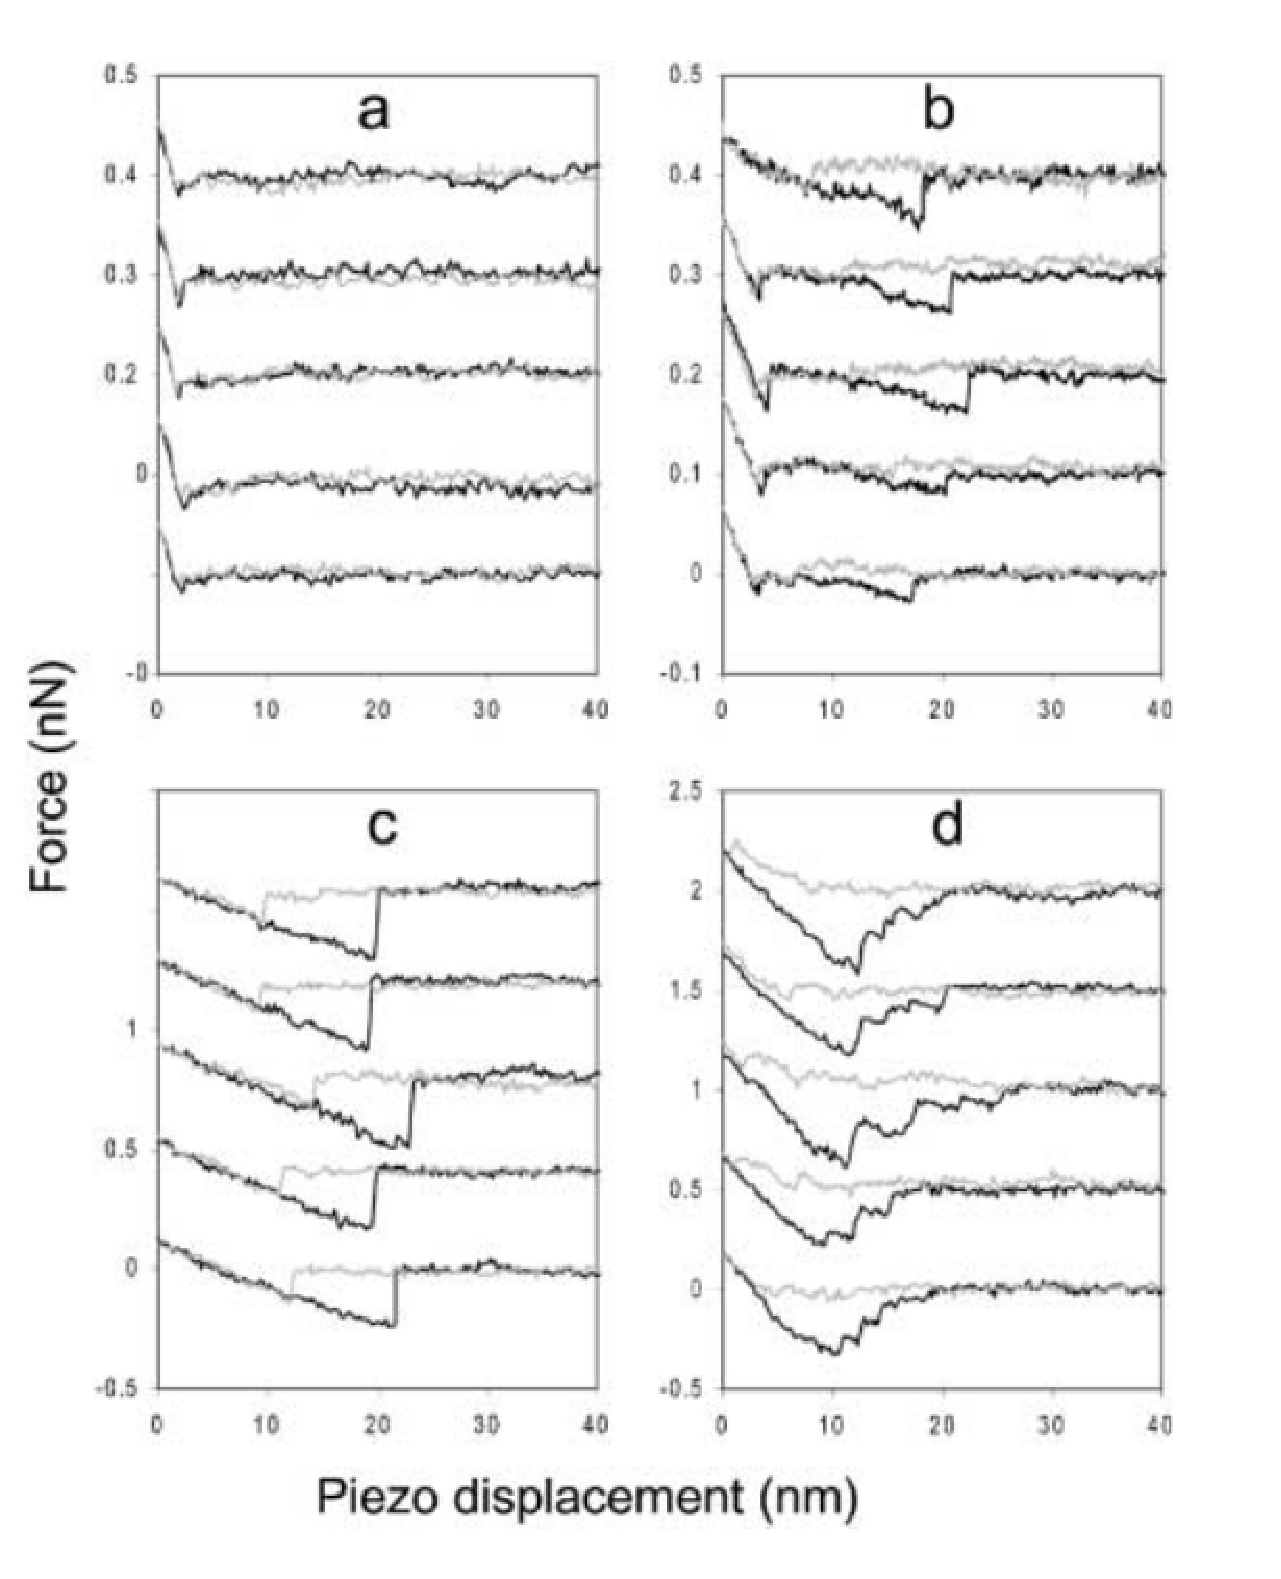
\includegraphics[height=1.9in, width=.8\textwidth]{experimental_pope.eps}
                \caption{}
                \label{fig:L12B6exp}
        \end{subfigure}
       
\floatsetup[figure]{font=1}
\caption{\small Melting profile for Force-induced DNA denaturations for DNA sequence L12B6.Fig(a) is the plot of fraction of open base pairs $l$ overall simulations and $f$ the fraction of open base pairs satisfying $\left<r_n\right>$ $>$ $r_{open}$ versus stretching force F. Fig(b) is the plot of helical rise h and twist angle $\theta$ against applied force F. Fig(c) is the plot of the average number of bubbles formed  $n_{bub}$ and the average  size of bubble $l_b$ against stretching force. Fig(d) is the plot of stretching force F versus extension. Fig(e) is the plot of  experimental force-extension relationship observed for single-molecules interactions between complementary oligonucleotides for the DNA sequence L12B6s obtained from the paper~\protect\cite{Pope:2001}\,.}
\label{fig:L12B6}    

\end{figure} 
%
\newpage
\section{Discussion}
 We applied the standard Metropolis algorithm to carry out our Monte Carlo simulation method to 
study the thermal and force-induced DNA denaturations phenomenon for the short DNA oligomer. It shows that the value of $l$obtained by averaging the fraction of open base pairs over the MC steps where the separation of at least one base pair is smaller than the dissociation threshold, well defined the meaning of double-stranded DNA ensemble. The value of  $f $ the fraction of open base pairs obtained from the condition $\left< r_{n}\right>$ $>$ $r_{open}$ grows with the denaturations of the bubbles so it's more convergence for the DNA sequences with a higher number of base pairs. For thermal DNA denaturations, our simulations result shows that $f$ for the DNA sequence L60B36 is more convergence than sequence L33B9 whereas for force-induced DNA denaturations L30B12 is more converged than L12B6. The thermal denaturation phenomenon suggests that in the given temperature range $40^\circ-100^\circ C$ the length of a bubble per base pair is directly proportional to the length of the DNA sequence. So, it suggests that short DNA sequences are more extended than the long DNA sequence. Our simulations result suggest that the force required to stretch the short DNA oligomer is inversely proportional to the length of the DNA sequence. It shows that the extension behavior of short DNA is also inversely proportional to the length of DNA. The lesser the DNA sequence, the more continuous and diverging is the DNA stretching phenomenon. Our both thermal and force-induced simulation result avoid the existence of the plateau region. The melting curve of Fig.\ref{fig:L12B6},\ref{fig:L20b8}, and \ref{fig:L30B12} shows that the boundness of the DNA sequence is inversely proportional to the number of the base pairs whereas the overstretched region is directly proportional to the length of base pairs. Therefore from the graph we found that $5\%$, $33\%$, and $46\%$ of the force are bounded, $32\%$, $24\%$, and $16\%$  of the force are in the stretched region, and $63\%$, $43\%$, and $38\%$  of the force are unbounded for L30B12, L20B8, and L12B6 respectively. Finally, the result of our simulation is in support that the cooperativity of the DNA stretching decreases with the decrease in the sequence of base pairs and BS transitions is the distinct characteristics of the infinitely long $\lambda$-DNA. We conclude that short DNA has a tendency to bear stresses and non-linearity in DNA stretching increases with the increase in the sequence of base pairs. Here, we studied the stretching behavior of the short DNA sequences. Interested candidates can also study the twisting behavior just adding twisting potential to the energy function. We have presented our results based on our simulation result and our knowledge and understanding of the helicoidal DNA. If any third party has a curiosity about our result and model, they are always welcome to provide the appropriate feedback to improve the model.
\newpage
%\nocite{*}
\bibliographystyle{plain}
\bibliography{references}
\biographypage
\end{document}
